\usepackage[T1]{fontenc}
\usepackage{textcomp}
\usepackage{amsfonts}
\usepackage{subfiles}% Mustervorlage für Abschlussarbeiten am LS DBIS
% Author: Alexander Stahl (stahlale@b-tu.de)
% Zuletzt aktualisiert am 10.02.2022

% Hinweis: Die Daten zur Arbeit speichern Sie in der Datei "data.tex".

% Diese Datei enthält Einstellungen und Paketimporte.
% Zur besseren Ordnung sollten Sie weitere Einstellungen bzw. Importe dieser Datei anfügen.

% Paketimporte
\documentclass[11pt,a4paper,german]{scrreprt}
\usepackage[utf8]{inputenc}  % Encoding
\usepackage{babel}  % Unterstützung verschiedener Sprachen
\usepackage{graphicx}  % Einbindung von Grafiken
\usepackage{amsmath}  % Verschiedene Symbole
\usepackage{amssymb}  % Verschiedene Symbole
\usepackage{latexsym}  % Verschiedene Symbole
\usepackage{booktabs}  % Schönere Tabellen
\usepackage{multicol}  % Flexiblere Tabellen
\usepackage[printonlyused]{acronym}  % Abkürzungsverwaltung
\usepackage{hyperref}  % Klickbare URLs, Titel und PDF-Metadaten
\usepackage{lipsum}  % Platzhaltertext (kann entfernt werden)
\usepackage[backend=bibtex,style=ieee]{biblatex}  % Moderne Literaturverwaltung
\usepackage{tikz} % Graphen zeichnen
\usetikzlibrary{positioning,shapes,shadows,arrows}

% Einstellungen
\hypersetup{
    colorlinks,
    citecolor=black,
    filecolor=black,
    linkcolor=black,
    urlcolor=black
}

\makeatletter

\newcommand\frontmatter{
	\cleardoublepage
	\pagenumbering{roman}}

\newcommand\mainmatter{
	\cleardoublepage
	\pagenumbering{arabic}}

\newcommand\backmatter{
  \if@openright
    \cleardoublepage
  \else
    \clearpage
  \fi
   }

\makeatother

% Laden der Literaturdaten
\addbibresource{quellen.bib}

% Definition der Dokumentendaten
% Zur besseren Kapselung wurde die Eingabe Ihrer Daten in diese Datei ausgelagert.
% Bitte einfach ausfüllen.

\newcommand{\TitelDeutsch}{Integrationstesten von GraphQL mittels Prime-Path Abdeckung} % Hier zentral angeben
\newcommand{\TitelEnglisch}{Integration testing of GraphQL using Prime-Path Coverage} % Übersetzten Titel auch angeben
\newcommand{\ArbeitsTyp}{Masterarbeit} % unzutreffendes hier löschen
\newcommand{\AuthorName}{Tom Lorenz} % Hier ändern
\newcommand{\MatrikelNr}{3711679}
\newcommand{\Studiengang}{Informatik M. Sc.}
\newcommand{\DatumThemenausgabe}{16.05.2023}
\newcommand{\DatumAbgabe}{31.8.2023}
\newcommand{\BetreuerEins}{Prof. Dr. rer. nat. Leen Lambers}
\newcommand{\BetreuerZwei}{Prof. Dr. rer. nat. Gerd Wagner} % Bitte immer akademische Titel angeben
\newcommand{\GutachterEins}{M. Sc. Lucas Sakizloglou} % Bitte immer akademische Titel angeben
  % In dieser Datei die Daten der Arbeit eingeben.

\titlehead{{Brandenburgische Technische Universität Cottbus-Senftenberg\\ Institut für Informatik\\ Fachgebiet Praktische Informatik/Softwaresystemtechnik}}
\subject{Masterarbeit\\ \vspace{0.5cm}\includegraphics[width=0.5\textwidth]{img/btu-logo.pdf}}
\title{\TitelDeutsch \\ {\normalsize \TitelEnglisch}}
\author{\AuthorName \\ MatrikelNr.: \MatrikelNr \\Studiengang: \Studiengang}
\date{\textit{Datum der Themenausgabe: \DatumThemenausgabe} \\ \textit{Datum der Abgabe: \DatumAbgabe}}
\publishers{1. Betreuer: \BetreuerEins \\ 2. Betreuer: \BetreuerZwei}

\hypersetup{pdfauthor={\AuthorName}}
\hypersetup{pdftitle={\TitelDeutsch}}

\tikzstyle{abstract}=[rectangle, draw=black, rounded corners, fill=blue!40, drop shadow,
text centered, anchor=north, text=white, text width=3cm]
\tikzstyle{comment}=[rectangle, draw=black, rounded corners, fill=green, drop shadow,
text centered, anchor=north, text=white, text width=3cm]
\tikzstyle{myarrow}=[->, >=open triangle 90, thick]
\tikzstyle{line}=[-, thick] % Header beinhaltet alle Einstellungen und Pakete. Bei Bedarf erweitern.

\begin{document}
  \frontmatter % kennzeichnet den vorderen Teil der Arbeit
  \maketitle % Titelseite generieren

  % Eidesstattliche Erklärung über Selbstständigkeit
  \section*{Eidesstattliche Erklärung}
Der Verfasser erklärt, dass er die vorliegende Arbeit selbständig, ohne fremde Hilfe und ohne Benutzung anderer als der angegebenen Hilfsmittel angefertigt hat.
Die aus fremden Quellen (einschließlich elektronischer Quellen) direkt oder indirekt übernommenen Gedanken sind ausnahmslos als solche kenntlich gemacht.
Wörtlich und inhaltlich verwendete Quellen wurden entsprechend den anerkannten Regeln wissenschaftlichen Arbeitens zitiert.
Die Arbeit ist nicht in gleicher oder vergleichbarer Form (auch nicht auszugsweise) im Rahmen einer anderen Prüfung bei einer anderen Hochschule vorgelegt oder publiziert worden.
Der Verfasser erklärt sich zudem damit einverstanden, dass die Arbeit mit Hilfe eines Plagiatserkennungsdienstes auf enthaltene Plagiate überprüft wird.

\vspace{2cm}

\noindent
\begin{tabular}{lcl}
  .................................... & \hspace{.4\textwidth} & ....................................\\
  Ort, Datum &  & Unterschrift

\end{tabular}


  % Automatische Generierung verschiedener Verzeichnisse
  % Inhaltsverzeichnis
  \tableofcontents
  \mainmatter
  % \mainmatter
  % Es folgt der Haupttext der Arbeit. Passen Sie die Überschriften der Kapitel entsprechend an.
  % Beachten Sie, dass die hier angegebene Gliederung nur ein Vorschlag ist.
  % Außerdem wird empfohlen, jedes Kapitel in eine eigene Datei auszulagern und hier nur mittels \input einzubinden.
  % Einleitung
  \chapter{Abstract}

Im Zuge der digitalen Transformation nimmt die Anzahl von Softwareanwendungen rasant zu und insbesondere durch das
Internet of Things und die generelle fortschreitende Vernetzung diverser Geräte nimmt in diesem Maße auch die Netzwerklast
zu.
Bisheriger Standard für Kommunikation von Geräten über das Internet waren REST-APIs diese haben jedoch gewisse
Limitierungen wie zum Beispiel: Ineffizienz durch Overfechting/Underfetching, Anzahl an Requests, Versionierung und Komplexität uvm.
Mit der Veröffentlichung von GraphQL in 2015 wurde ein Konkurrent zu REST in das Leben gerufen der diese Probleme beheben kann.
Durch GraphQL lässt sich insbesondere die Netzwerklast reduzieren da eine GraphQL-Request, im Gegensatz zu REST, mehrere Anfragen in einer
einzigen HTTP-Request zusammenfassen kann und dabei auch nur die wirklich gewünschten Daten überträgt.
Dadurch, dass jedoch die wachsende Anzahl von Softwareanwendungen auch in immer kritischere Bereiche des Lebens vordringt, ist es
enorm wichtig die Qualität der Software sicherzustellen.
Eine Methodik zum Sicherstellen der korrekten Funktionalität von Software ist das Testen von Software im Sinne von Validierungstests die sicherstellen sollen,
dass die Software vorher definierte Szenarien nach Erwartung behandelt.
Für REST-APIs existieren zahlreiche Tools die solche Validierungstests automatisch übernehmen können wohingegen es noch einen Mangel
an Tools dieser Art für GraphQL gibt.
Im Rahmen der IEEE/ACM 2021 wurde ein Paper veröffentlicht, dass eine Methode vorstellt wie GraphQL-APIs mithilfe von
"Property-based" Tests automatisch getestet werden können.
"Property-based" bzeieht sich darauf, dass die Eigenschaften eines Objektes genutzt werden um diese zu testen.
Diese Methode generiert zufällig Tests und bietet so eine Möglichkeit, Fehler zu entdecken und
generell erstmal eine Grundlage an Tests zu schaffen frei nach dem Motto: "lieber irgendwelche Tests als gar keine Tests".
Die zufallsbasierte Testgenerierung weist allerdings einige Schwachstellen auf.
So kann Sie nicht garantieren, dass die API zu jeder Zeit eine gute Coverage hat denn es können einzelne Routen der API
komplett ausgelassen werden.
Es sind Testszenarios denkbar, die sehr viele false-positives durchlassen \& somit die Qualität der Software nicht ausreichend sicherstellen können.
GraphQL ermöglicht außerdem einen potentiell unendlichen Suchraum für die Tests.
Um diesem Problem zu entgehen wurde ein einfaches rekursions-limit definiert was jedoch dazu führt, dass die Testabdeckung nur bis zu einem
bestimmten Grad überhaupt reichen kann.
Längere Pfade die mit GraphQL definiert werden können, werden deshalb niemals getestet.

Mit dieser Arbeit soll ein anderer Ansatz für die automatisierte Testgenerierung untersucht werden.
Hierbei soll untersucht werden, inwiefern Graphcoverage auf GraphQL angewendet werden kann zur Generierung von
Tests.
Mithilfe von einem allgemeinen Graphalgorithmus, der sonst zur Kontrollflussgraphen Analyse benutzt wird, wollen wir zeigen,
dass es möglich ist mit einem iterativen Verfahren GraphQL zu testen.
Wir versprechen uns von den Graphcoverage-Algorithmen einer verlässliche und sichere Generierung von Tests die
einerseits effizient jegliche Methoden abdecken und andererseits die Anzahl der Tests minimal hält.
Um die Methodik zu validieren werden am Ende beide Tools einem Experiment unterzogen um zu sehen ob die hier
vorgestellte Methode eine Verbesserung erzielen kann.


%Mit zunehmender Popularität von GraphQL werden Tools benötigt, die Sicherheit, Zuverlässigkeit und korrekte Funktionalität
%von GraphQL verifizieren und validieren können.
%Durch die starke Typisierung von GraphQL lässt sich der Testraum jedoch sehr schön eingrenzen.
%Aktuell gibt es aber noch Einschränkungen an Testtools für GraphQL-Apis, insbesondere im Bereich der automatischen Testanalyse.
%Im Paper \" Automatic Property-based Testing of GraphQL APIs \" (Quelle hinzufügen) wurde sich mit einem automatischen
%Testverfahren für Integrationstest für GraphQL-API's beschäftigt.
%Hierbei wurde der Ansatz der zufallsbasierten Testgenerierung genutzt, um Tests zu generieren.
%Die zufallsbasierte Testgenerierung weist allerdings einige Schwachstellen auf.
%So kann Sie nicht garantieren, dass die API zu jeder Zeit eine gute Coverage hat.
%Es sind Testszenarios denkbar, die sehr viele false-positives durchlassen \& somit die Qualität der Software nicht ausreichend sicherstellen können.
%GraphQL ermöglicht außerdem einen potentiell unendlichen Suchraum für die Tests.
%Um diesem Problem zu entgehen wurde ein einfaches rekursions-limit definiert was jedoch dazu führt, dass die Testabdeckung
%wieder nicht garantiert sichergestellt werden kann.
%Mithilfe von einem allgemeinen Graphalgorithmus, der sonst zur Kontrollflussgraphen Analyse benutzt wird, wollen wir zeigen,
%dass es möglich ist mit einem iterativen Verfahren GraphQL zu testen.
%Hierbei werden die Probleme des unendlichen Suchraumes und der zufälligen Testüberdeckung systematisch und effizient gelöst.
%Um zu validieren, dass unsere Methode eine Verbesserung bietet werden einige Experimente durchgeführt in denen wir
%verschiedene Metriken vergleich hierbei unter anderem: Anzahl der generierten Tests, Testabdeckung der Schnittstelle und
%gefundene Fehler.


%Diese Arbeit hat allerdings einige Limitierungen wie zum Beispiel ein Rekursionslimit, dass die Größe der zu testenden
%API stark limitiert und einen Fokus auf zufallsbasierte Testgenerierung.
%In dieser Arbeit soll auf die Methode des \" Automatic Property-based Testing of GraphQL APIs \"
%eingegangen werden und mit einem anderen, strukturierteren Ansatz verbessert werden.
%Denn GraphQL definiert eine sehr stark typisierte Schnittstelle welche mithilfe von Graphalgorithmen untersucht werden kann.
%Ziel dieser Arbeit ist es, Graphüberdeckungen nach \cite{software-testing} zu untersuchen und Algorithmen zu implementieren
%die zu einer optimalen bzw hinreichenden Überdeckung eines Graphen führen.

%Hierzu soll der PrimePath Algorithmus, der klassischerweise für Graphüberdeckung in Kontrollflussgraphen verwendet wird, auf
%dieses Problem angepasst werden und evaluiert werden, inwiefern dieser zu einer Lösung des Problems beiträgt.
%Hierzu folgt am Ende ein Vergleich zwischen der ursprünglichen und neu entwickelten Methode.


%alter Text:
%Allerdings bietet diese Arbeit ein Verbesserungspotential, welches in dieser Arbeit untersucht und implementiert werden soll.
%Im konkreten handelt es sich bei dem automatischen Testverfahren um ein Verfahren, das ein GraphQL-Schema aufgrund seiner
%Struktur rekursiv untersucht und hieraus tests generiert.
%Hierbei wird zwar Rücksicht auf die spezielle Graphstruktur genommen allerdings werden spezifische Grapheigenschaften nicht ausgenutzt, um die Tests zu verbessern.
%Dabei sind diverse Arbeiten publiziert worden die sich mit Graphenüberdeckung beschäftigen welche auch
%Algorithmen anwenden, die zyklische Strukturen gut überdecken.
%Ziel dieser Arbeit ist es, dieses Wissen über Graphüberdeckung zu nutzen indem besagte GraphAlgorithmen
%den rekursiven Suchalgorithmus des Papers ersetzen.
%Hierdurch erhoffen wir uns eine Verbesserung der Test-Coverage.
  %! Author = Tom
%! Date = 07.12.2022
\chapter{Einleitung}

In diesem Kapitel wird an das Thema und die Motivation dieser Arbeit herangeführt.
Außerdem wird definiert, welche Ziele diese Arbeit erreichen soll und eine grobe Übersicht über die
Kapitelstruktur gegeben.

\section{Motivation}

Mit einer steigenden Nutzung von GraphQL wird es immer wichtiger, geeignete Tests für GraphQL-API's zu entwickeln damit eine
gute Softwarequalität sichergestellt werden kann.
Tests können manuell geschrieben oder automatisch generiert werden.
Während bei Unit-Tests für einzelne Methoden der Programmierer frei entscheiden kann, ob er die Tests selbst schreiben will
oder doch eher von einem Tool generieren lassen will sind bei Integrations-Tests die Testräume teilweise so groß, dass ein
manuelles Schreiben dieser Tests einerseits fehleranfällig aber auch schlicht zu langwierig ist.
Für REST-APIs existieren schon automatische Integrationstesttools wie zum Beispiel: EvoMaster \cite{evo-master} , QuickREST \cite{karlsson2019quickrest} oder RESTTESTGEN \cite{rest-test-gen}.
GraphQL-APIs haben leider noch einen Mangel an solchen automatischen Testtools.
Im Rahmen der IEEE/ACM 2021 wurde mit ''Automatic Property-based Testing of GraphQL APIs''\cite{property-based-testing} eine Methode vorgestellt die diesen Mangel angehen soll.
Ergebnis der Arbeit war hierbei ein Prototyp der die vorgestellte Methode umsetzten sollte.
Die vorgestellte Methode bezieht sich auf ''Property-based Testing'' wobei diese gleichzusetzen ist mit ''Random Testing'' \cite{property-based-testing}[vgl. 2.B]
Durch die starke Typisierung und Schema-Definition, welche prinzipiell ein Graph ist, lässt sich in GraphQL
sehr einfach auswerten welche Anfragen nun zulässig sind.
Die hier vorgestellte Methode nutzt den Fakt, dass zum Beispiel alle möglichen Anfragen immer im Query-Knoten
beginnen müssen und somit alle weitergehenden Felder im Schema innerhalb des Query-Knoten definiert sein müssen.
Da die Definition des Schemas der eines Graphens entspricht ist jedoch der mögliche Suchraum potentiell unendlich da GraphQL
Zyklen innerhalb des Graphens erlaubt.
Der unendliche Suchraum wurde durch ein Rekursionslimit begrenzt allerdings wird so eine schlechtere Test-Coverage erreicht.
\newpage
Die bisher entwickelte Methode funktioniert auf folgende Weise:

\begin{center}
    \includegraphics[width=\textwidth,height=\textheight,keepaspectratio]{content/einleitung/toolchain}
    \caption{Methode von~\cite{property-based-testing}}
\end{center}

wobei neben dem vorher erwähnten Rekursionslimit außerdem Punkt 6. ''Verify response Properties'' kritisch
zu betrachten ist da die Auswertung wirklich nur auf die Properties schaut.
Dies bedeutet, dass ein zurückgegebens Objekt nur auf seinen Typ überprüft wird aber nicht, ob seine tatsächlichen Rückgabewerte, die exakt erwartet sind.
Hierdurch können false-positives entstehen.

Die vorgestellte Methode wollen wir verbessern durch Änderung einiger Ansätze.
Hierbei sollen Graphcoverage-Algorithmen zum Einsatz kommen, die mit iterativen Verfahren auch zyklische Graphen ideal
überdecken können und dabei immer verlässlich arbeiten, sodass die generierten Tests stets für vergleichbare Ergebnisse sorgen und nicht
davon abhängig sind, dass der Zufall eine gute Überdeckung liefert.
Zusammenfassend sei gesagt, dass bei der Testgenerierung und Testauswertung Verbesserungen möglich sind und dies Gegenstand dieser Arbeit sein soll.

\section{Umsetzung}

Zuallererst wird in dieser Arbeit etwas Theorie definiert und in Bezug gesetzt.
Wir beginnen damit die Graphentheorie als mathematisches Konzept zu definieren denn dieses liegt GraphQL zugrunde.
Darauffolgend kommt eine kleine Einführung in GraphQL und dann bilden wir schon die Schnittstelle von GraphQL zur Graphentheorie.
Sobald diese Verbindung erfolgt ist können wir uns dem eigentlichen Problem widmen: Wie kann man mithilfe von Graphcoverage-Algorithmen
Tests generieren?
Hierfür erfolgt ein letzter Theorie-Exkurs über Software-Tests.
Mit diesen Grundlagen schaffen wir es dann unsere Methode zu entwickeln und können Sie auch mit ''Automatic Property-based Testing of GraphQL APIs''\cite{property-based-testing}
vergleichen.
Unsere Methode wird konzeptionell vorgestellt und dann folgen einige Implementierungsdetails sowie ein Vergleich beider Tools durch Experimente.
Abschließen wird die Arbeit mit einem Ausblick für zukünftige Arbeit und einem Fazit über unsere erreichten Verbesserungen.

  % Hauptteil
  \chapter{verwandte Arbeiten}
\label{relatedWork}

Da GraphQL eine stetig wachsende Beliebtheit verzeichnet \cite{graphql-growing-report}[vgl. Language Features] steigt auch der Bedarf und das Interesse an Testmethoden.
Aktuell gibt es für GraphQL noch eine Lücke an produktionsreifen Testtools, insbesondere automatischen Testtools.
Eine wachsende Anzahl an research-tools beziehungsweise untersuchten Methoden ist allerdings zu verzeichnen.
In diesem Kapitel sollen diese Methoden benannt werden und Verwandheiten, Unterschiede oder thematische Überschnitte von dieser und anderen Arbeiten benannt werden.

\section{Property Based Testing}

In ''Automatic Property-based Testing of GraphQL APIs''\cite{property-based-testing} wird der Ansatz des Property-based Testing verfolgt, um Integrationstests zu erstellen.
Property-based Testing ist laut dem Paper heute Synonym mit "Random Testing"\cite{property-based-testing}[vgl. 2B] wobei zufällig hierbei meint,dass die Eingabedaten und Routen zufällig generiert werden.
Wie Eingangs schon erwähnt, hat die Methode einige Limitierungen.
Wir wollen diese hier noch einmal aufgreifen und vertiefen.
Der allgemeine Funktionsablauf der Testgenerierung laut Paper ist wie folgt:

\begin{center}
    \begin{itemize}
        \item[1.] Vom Schema, generiere Typ-Spezifikationen
        \item[2.] Generiere einen Generator der zufällig eine Liste an Query-Objekten erstellen kann
        \item[3.] Generiere n Querys
        \item[4.] Transformiere die Queries in GraphQL-Format
        \item[5.] Führe die Queries auf dem SUT (system under test) aus
        \item[6.] Evaluiere die Ergebnisse auf ihre Properties
    \end{itemize}[\cite{property-based-testing}[vgl. 3. Proposed Method]]
\end{center}

Insbesondere Punkt 2. und Punkt 6. weisen Verbesserungsbedarf auf.
Punkt 2 wird auch der Hauptunterscheidungspunkt beider Arbeiten sein, denn hier sind dann zwei gänzlich unterschiedliche Konzepte am Werk.
Dieser ist beim Property-Based Testing nämlich ein Query-Generator der mithilfe der Clojure-Bilbiothek Serene\cite{clojureserene}
Clojure.Specs\cite{clojurespec} generiert und diese Clojure.Specs\cite{clojurespec} dann nutzt um mit der Clojure-Bilbiothek Malli\cite{clojuremalli} dann Daten für die Testqueries zu generieren.
Unsere herangehensweise wird sich hiervon gänzlich unterscheiden.
Im Sinne von Property-based Testing ist diese Herangehensweise allerdings eine sehr sinnvolle gewesen da Malli\cite{clojuremalli} de-facto Standard
für Property-based Testing in der Clojure-Welt ist.
Geht man jedoch davon aus, dass das Ziel eine ideale Überdeckung des Graphens jeder größe und jeder Struktur ist, so
ist diese herangehensweise nicht die beste.\cite{property-based-testing}[vgl. 3C]
Laut dem Paper gilt ''ein größeres und mehr rekursives (GraphQL)-Schema würde nicht skalieren und der (zufällig) iterative Ansatz ist besser als eine Breitensuche''\cite{property-based-testing}[vgl. 3C].
Diese Behauptung betrachten wir als falsch und behaupten, dass es besser möglich ist.
Dies zu zeigen bleibt Gegenstand der folgenden Arbeit.


\section{heuristisch suchenbasiertes Testen}

EvoMaster\cite{evo-master} ist ein Open-Source Tool welches sich automatisiertes Testen von Rest-APIs und GraphQL APIs zur Aufgabe gemacht hat.
Aktuell kann durch EvoMaster sowohl WhiteBox Testing als auch BlackBox Testing durchgeführt werden jedoch ist ein
Whitebox Test mittels Vanilla-EvoMaster nur für Rest-APIs möglich die mit der JVM lauffähig sind.
Im Paper ''White-Box and Black-Box Fuzzing for GraphQL APIs''\cite{belhadi2022whitebox} wurde ein System on-Top für EvoMaster
erstellt welches GraphQL Tests generieren kann.
Hierbei soll sowohl WhiteBox als auch BlackBox Testing möglich sein.
Das erstellte Framework in diesem Paper arbeitet nach folgendem Prinzip:

\begin{center}
    \includegraphics[width=\textwidth,height=\textheight,keepaspectratio]{content/hauptteil/relatedWork/evomaster_framework}
\end{center}

WhiteBox Testing ist möglich insofern Zugang zum GraphQL-Schema und zum Source Code der API gegeben ist.
Andernfalls ist nur BlackBox Testing möglich.
Zur Testgenerierung wird ein genetischer Algorithmus genutzt welcher die Tests generiert.
Wie dieser genetische Algorithmus genau funktioniert kann im Paper selbst nachgelesen werden\cite{belhadi2022whitebox}.
Im Vergleich mit unserer geplanten Arbeit mittels des Prime-Path-Algorithmus ergeben sich einige Unterschiede, diese sind
unter anderem: Nutzung eines evolutionären Algorithmus Many-Independent-Objective (MIO).
Im Paper selbst wird davon ausgegangen, dass andere evolutionäre Algorithmen unter Umständen passender wären als der MIO Algorithmus
für die Testgenerierung.
Jedoch ist ein evolutionärer Algorithmus auch immer ein stochastisch, heuristisch sich dem Optimum annähernder Algorithmus. (Beleg hierfür)
Im Gegensatz dazu ist der Ansatz dieser Arbeit ein iterativer Algorithmus der ideale Überdeckungen auf direkte Art bietet
und im ersten Durchlauf direkt sein ideales Ergebnis ermittelt.
Die ideale Lösung bezieht sich hierbei auf bestimmte Code-Coverage Kriterien die durch unseren Algorithmus erfüllt werden.
Inwiefern der evolutionäre Algorithmus diese Kriterien erfüllt bleibt offen, es ist jedoch davon auszugehen, dass er sich einer idealen Lösung dieser Kriterien nur
annähert da er eben ein stochastischer Algorithmus ist. (beleg oder Quelle)

\section{Deviation Testing}

Da GraphQL dynamisch auf Anfragen reagiert und es somit möglich ist, in seiner Anfrage einzelne Felder mit einzubeziehen
oder auch auszuschließen ist dies im Grunde genommen ein einzelner Test-Case.
Im Paper \" Deviation Testing: A Test Case Generation Technique for GraphQL APIs" wird diese Gegebenheit benutzt und
aus einer selbstdefinierten Query werden hier einzelne Test-Cases gebildet. Ein solcher Test macht je nach Implementierung
der GraphQL-Resolver druchaus Sinn, da im Backend Felder durchaus zusammenhängen können und es Bugs geben kann wenn
Resolver fehlerhaft definiert sind. z.B. könnte folgende Definition zu solchen Fehlern führen:

(hier BSP mit Code einfügen)

Da Deviation Testing jedoch nur bestehende Tests erweitert um mögliche Felder mitzutesten werden hier keine neuen Tests generiert.
Durch Deviation Testing werden bestehende Tests nur erweitert allerdings muss eine Edge-Coverage gegeben sein damit diese Arbeit
ein zufriedenstellendes Ergebnis erzeugt. Eine Edge-Coverage in einem komplexen Graphen ist allerdings sehr wahrscheinlich
schwer umsetzbar mit manuellem Test schreiben. Eine Paarung von Edge-Coverage mit Deviation-Testing wäre sicherlich Interessant.
Genau so wäre es interessant Deviation Testing als Teil unserer Arbeit zu nutzen indem mit diesem Tool die Tests erweitert werden.
(initialer Plan war es, einfach immer alle Felder eines Nodes zu testen, hierdurch wäre es möglich auch alle Varianten noch zu testen)

\section{Query Harvesting}

Klassisches Testen von Anwendungen beeinhaltet, dass möglichst das komplette System getestet wird bevor es verwendet wird.
Im Paper "Harvesting Production GraphQL Queries to Detect Schema Faults" wird ein gänzlich anderer Ansatz verfolgt.
Hierbei ist es nicht wichtig die gesamte GraphQL-API vor der Veröffentlichung zu testen sondern
echte Queries die in Production ausgeführt werden zu sammeln.
Der Ansatz der hierbei verfolgt wird begründet sich daraus,
dass ein Testraum für GraphQL potentiell unendlich sein kann und es sehr wahrscheinlich ist, dass nur ein kleiner
Teil der API wirklich intensiv genutzt wird, sodass auch nur dieser Teil wirklich stark durch Tests abgedeckt werden muss.
AutoGraphQL läuft hierbei in zwei Phasen wobei in der ersten Phase alle einzigartigen Anfragen geloggt werden.
In der zweiten Phase werden dann aus den geloggten Anfragen Tests generiert.
Hierbei wird für jede geloggte Query genau ein Test-Case erstellt.
Bei dieser Art des Testens wird insbesondere darauf Wert gelegt, dass es keine Fehler im GraphQL Schema gibt.
Dies ist ein wichtiger Teil um GraphQL-API's zu testen allerdings noch kein vollständiger Test denn hier wird außer Acht gelassen,
dass eine Query konform zum GraphQL-Schema sein kann aber trotzdem falsch indem zum Beispiel falsche Daten zurückgegeben werden
durch falsche Referenzierung oder ähnlichem.
In dem zu entwickelndem Tool sollten alle Querys die von AutoGraphQL geloggt werden auch berücksichtig werden da sie durch
den Prime-Path Algorithmus auch ermittelt werden.
Es kann allerdings sinnvoll sein AutoGraphQL als Monitoring-Software mitlaufen zu lassen und weitere etwaige Fehler hiermit zu loggen
und automatisch daraus Test-Cases erstellen zu können damit zukünftig keine Fehler dieser Art mehr passieren.

\section{Vergleich der Arbeiten}
Folgender Vergleich soll die verwandten Arbeiten noch einmal kurz einordnen.

\newcolumntype{C}{>{\Centering\arraybackslash}X}
\begin{center}
    \begin{table}[!hbt]
        \begin{tabularx}{\textwidth}{|C|C|C|C|C|C|}
            \hline
            \textbf{ Arbeit / Kriterium} & \textbf{Property Based Testing} & \textbf{heuristisch suchenbasiertes Testen} & \textbf{Deviation-Testing} & \textbf{Query Harvesting} \\
            \hline
            Generierungsart & Zufallsbasierte Routengenerierung & Heuristische Suche & Erweiterung von bestehenden Tests & Tracken von Querys und daraus Tests generieren \\
            \hline
            Überdeckung & Zufällig, stark abhängig von Schema  & abhängig ob Zugang zu Source Code, Zufällig aber optimaler & stark abhängig von selbst geschriebenen Tests  & stark Abhängig von User-requests  \\
            \hline
            Orakel & simples Raten & mit Source Code: Analyse & Aus entwickelten Tests &  Aus gestellten Querys \\
            \hline
            Ausführzeit & vor Prod & vor Prod & vor Prod & Verifikation / Wartung \\
            \hline
            Use-Case & allgemeines Testen & allgemeines Testen & allgemeines Testen & Testen bei Code-Änderung \\
            \hline
        \end{tabularx}
    \end{table}
\end{center}

\section{Andere Arbeiten}
Hier ist eine kurze Übersicht über andere Arbeiten, dieses Kapitel ist sehr unwahrscheinlich in einer Abgabeversion.
Es dient eher als Notizensammlung in einer hübscheren Form.

\subsection{Empirical Study of GraphQL Schemas}
Eine umfangreiche Untersuchung von Praktiken in GraphQL. Unterteilt in verschiedene Metriken wie z.B.
Anzahl der Objekttypen, Querys etc.
Interessant ist allerdings die Untersuchung von zyklischen Schemas. Insbesondere, wie groß diese Zyklen
werden können und wie sie begrenzt werden. Dies ist interessant für spätere Auswertungen. Allerdings bringt
diese Arbeit nicht viel für das direkte Testen.

\subsection{LinGBM Performance Benchmark to Build GraphQL Servers}
Eher eine Untersuchung wie GraphQL-APIs unter Last performen bzw. wie Effizient sie sind.
Der benutzte Query-Generator kann interessant sein aber es ist schwer einschätzbar wie dieser in unserem Kontext genutzt werden
kann.

\subsection{GraphQL A Systematic Mapping Study}
Richtig gute Übersicht wie GraphQL "Unter der Haube" funktioniert




  \chapter{Grundlagen / Theorie}

Das automatisierte Testen von GraphQL-API's erfordert ein spezifisches Domänenwissen in verschiedenen Teilbereichen der
Informatik und Mathematik. Dieses Domänenwissen wird in den folgenden Abschnitten aufgrundlage zweier Lehrbücher erarbeitet
und in Kontext gesetzt. Wissen über die Graphentheorie wird benötigt, da GraphQL eine Implementierung von graphenähnlichen Strukturen
ist und wir somit Algorithmen darauf anwenden können. Die mathematische Formalisierung hilft hierbei dann insbesondere
bei der Beweisführug für eine allgemeine Termination der zu entwickelnden Algorithmen.
Desweiteren ist es nötig sich bewusst zu machen, welche Arten des Testens von Software es gibt und warum wir bestimmte
Methoden hier eher nutzen als andere.
Im konkreten ist das Theorie-Kapitel so strukturiert, dass erst einmal die mathematischen Grundlagen der Graphentheorie
vermittelt werden und im Anschluss dazu wird eine Beziehung zwischen GraphQL \& Graphentheorie hergestellt.
Mit der Beziehung können wir dann zeigen, dass Graphalgorithmen auch bei GraphQL anwendbar sind.
Mit diesen Grundlagen können wir dann zeigen, dass verschiedene Überdeckungsalgorithmen zur idealen Testgestaltung genutzt werden können
wobei hier natürlich definiert werden muss, was überhaupt eine Testüberdeckung ist und wann diese "ideal" ist.


  \section{Graphentheorie}
\label{sec:graphentheorie}

Da GraphQL es ermöglicht, dass komplexe Beziehungen innerhalb eines Datenmodells in Form von Graphen modelliert werden~\cite[vgl. Modelling with Graph(QL)]{graphqlgraphtheory}
benötigt man die Graphentheorie, da diese Methoden liefert, um Graphen zu definieren und zu analysieren.
Des Weiteren sind die Testabdeckungskriterien, die später genutzt werden, eng mit der Graphentheorie verbunden.
Die folgenden Absätze werden eher theoretisch gehalten.
Die Zusammenhänge zwischen der Graphentheorie und Testen von GraphQL-APIs werden sich jedoch später erschließen.

\subsection{Ungerichteter Graph}

Ein Graph ist ein mathematisches Modell.
Es kann dazu verwendet werden, Beziehungen zwischen Objekten darzustellen.
Nach~\cite{graphentheorie} ist ein ungerichteter Graph wie folgt definiert:

\begin{definition}
    Ein ungerichteter Graph ist ein Paar $\textrm{G = (V, E)}$ zweier disjunkter Mengen mit E $\subseteq$ V^2
    \label{graphdef}
\end{definition}\cite[vgl. S.2 0.1 Graphen]{graphentheorie}
\\
\\
Die Elemente der Menge $V$ heißen Knoten (Vertices).
Verbindungen zwischen den Knoten sind Elemente der Menge $E$ und diese nennt man Kanten (Edges).
In dieser Definition spielt die Ordnung der Elemente von E keine Rolle, daher nennt man solche Graphen auch ungerichtete Graphen.
Um Graphen darzustellen, gibt es verschiedene Ansätze.
Der geläufigste Ansatz ist es, Knoten als Punkte und Kanten als Verbindungslinien zu zeichnen.
Häufig wird auch eine Adjazenzmatrix genutzt, bei dieser wird mit $0,1$ aufgeschlüsselt, welche Knoten eine Verbindung haben.
Bei $0$ existiert keine Kante zwischen den Knoten und bei $1$ existiert eine.

\begin{example}
    Ein Graph sei definiert mit $V = \{ 1, 2, 3 \}$ und $E = \{(1,1), (1,2), (1,3) \}$ \\
    Mögliche Darstellungen des Graphen sind in Abbildung~\ref{zeichnung} und~\ref{adjam} gezeigt.
    \label{exmgr}
\end{example}
    \begin{figure}[h!]
        \centering
        % Linke Seite: Code
        \begin{minipage}{0.45\textwidth}
            \centering
            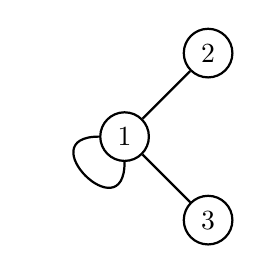
\begin{tikzpicture}[node distance={15mm}, thick, main/.style = {draw, circle}]
                \node[main] (1) {$1$};
                \node[main] (2) [above right of=1] {$2$};
                \node[main] (3) [below right of=1] {$3$};
                \draw (1) to [out=180,in=270,looseness=5] (1);
                \draw (1) -- (2);
                \draw (1) -- (3);
            \end{tikzpicture}
            \caption{Gezeichneter Graph}
            \label{zeichnung}
        \end{minipage}
        \hfill
        \begin{minipage}{0.45\textwidth}
            \centering
            \begin{array}{c|ccc}
                & 1 & 2 & 3 \\
                \hline
                1 & 1 & 1 & 1 \\
                2 & 0 & 0 & 0 \\
                3 & 0 & 0 & 0 \\
            \end{array}
            \caption{Adjazenzmatrix}
            \label{adjam}
        \end{minipage}
    \end{figure}

\subsection{Gerichteter Graph}

Gerichtete Graphen sind die Grundlage vieler Überdeckungskriterien~\cite[vgl. 2.1 Overview]{software-testing}.
Daher werden sie hier definiert.

\begin{definition}
    Ein gerichteter Graph ist ein Paar $\textrm{G = (V, E)}$ zweier disjunkter Mengen mit zwei Funktionen
    init: E \textrightarrow V und ter: E \textrightarrow V, die jeder Kante e eine Anfangsecke init(e) und eine
    Endecke ter(e) zuordnen~\cite[S.26 0.10 Verwandte Begriffsbildungen]{graphentheorie}.
    \label{gerichtetergraphdef}
\end{definition}

Bei einem gerichteten Graphen ist die Sortierung der Kantenpaare wichtig.
Die Funktionen $init$ und $ter$ können nämlich am einfachsten durch die Sortierung der Elemente eines Kantenpaares umgesetzt werden.
Hierbei ist das erste Element des Kantenpaares die Anfangsecke und das zweite Element ist die Endecke.
Die Kanten in einem gerichteten Graphen werden mit einem Pfeil gezeichnet.
Dabei zeigt der Pfeil stets in Richtung Endecke.
Der in Beispiel~\ref{exmgr} definierte Graph ist als gerichteter Graph in Abbildung~\ref{graphexample} gezeigt.

\begin{figure}[H]
    \begin{center}
        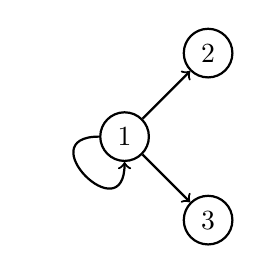
\begin{tikzpicture}[node distance={15mm}, thick, main/.style = {draw, circle}]
            \node[main] (1) {$1$};
            \node[main] (2) [above right of=1] {$2$};
            \node[main] (3) [below right of=1] {$3$};
            \draw[->] (1) to [out=180,in=270,looseness=5] (1);
            \draw[->] (1) -- (2);
            \draw[->] (1) -- (3);
        \end{tikzpicture}
    \end{center}
    \caption{ein gerichteter Graph}
    \label{graphexample}
\end{figure}

\subsection{Gewichteter Graph}

Für die spätere Entwicklung des Testentwurfs ist es wichtig, gewichtete Graphen zu definieren.
Zuvor wurde eine Kante in Definition~\ref{graphdef} und Definition~\ref{gerichtetergraphdef} als ein Tupel $(x, y)$ eingeführt.
Ein gewichteter Graph weist jeder Kante ein Kantengewicht zu, dies ist im Allgemeinen eine positive, reelle Zahl~\cite[vgl. S. 251]{graphentheorie3}.

\begin{definition}
    Ein Graph G = (V,E) mit einer Abbildung g : E \textrightarrow $\mathbb{R}_{>0}$ heißt gewichteter Graph.
    Die Abbildung g heißt Gewichtsfunktion. Für $e \in E$ heißt g(e) das Gewicht von e.
    Das Gewicht von G ist die Summer der Gewichte aller Kanten, g(G) = \sum_{e \in G} g(e).\\
    \cite[vgl.~Definition~6.1~S.~251]{graphentheorie3}
    \label{gewichtetergraph}
\end{definition}
\\
\\
Für spätere Anwendungszwecke muss die Definition jedoch ein wenig allgemeiner gefasst werden.
Die Felder eines GraphQL-Typens sollen später als Gewicht genutzt werden, um Tests zu entwerfen.
Um dies zu erleichtern, soll die Definition~\ref{gewichtetergraph} verallgemeinert werden durch eine Anpassung der Gewichtsfunktion.
Die neue Definition soll vorerst \textit{allgemein gewichteter Graph} genannt werden.

\begin{definition}
    Ein Graph G = (V,E) mit einer Abbildung g: E \textrightarrow X heißt allgemein gewichteter Graph.
    Die Menge X ist frei wählbar.
    \label{allgemeingewichtetergraph}
\end{definition}

\subsection{Pfad}

Ein Pfad, oft auch Weg genannt, ist eine Sequenz von Knoten, die nachfolgend durch Kanten miteinander verbunden sind~\cite[vgl. S. 7 0.3]{graphentheorie}.

\begin{definition}
    Ein Weg ist ein nicht leerer Graph P = (V,E) der Form $V = {x_{0}, x_{1}, ..., x_{k}}$ und $E = {x_{0}x_{1}, x_{1}x_{2}, \ldots, x_{k-1}x_{k}}$ wobei die $x_{i}$
    paarweise verschieden sind~\cite[vgl. S. 7]{graphentheorie}.
\end{definition}

Ein Weg wird oft durch die Folge seiner Knoten beschrieben also $P=x_{0} x_{1} \ldots x_{k}$ \cite[vgl. S.7]{graphentheorie}
Die Länge eines Weges ist die Anzahl der Kanten, die dieser besucht~\cite[vgl. S. 7]{graphentheorie}.
In gewichteten Graphen ist das Gewicht eines Pfads die Summe aller Gewichte der einbezogenen Kanten~\cite[vgl. 7.2 kürzeste Wege]{graphentheorie3}.

\begin{example}
    Es sei ein Graph G definiert mit V = $\{n1,n2,n3,n4,n5,n6,n7,n8\}$ und E = $\{(n1,n2),(n2,n3),(n3,n4),(n4,n1),(n2,n5),(n3,n6),(n5,n7),(n6,n8)\}$.
    Ein möglicher Pfad von Knoten $n1$ zu $n8$ ist der Pfad $p = \{(n1, n2), (n2, n3), (n3, n6), (n6, n8)\}$.
    Der Pfad p ist in Abbildung~\ref{pfadbsp} rot markiert \\ \\
\end{example}

\begin{figure}[H]
    \begin{center}
        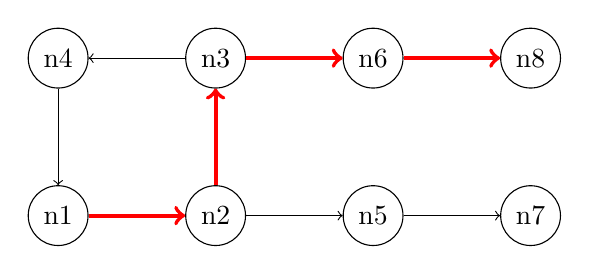
\begin{tikzpicture}
            \node[circle, draw] (n1) at (0,0) {n1};
            \node[circle, draw] (n2) at (2,0) {n2};
            \node[circle, draw] (n3) at (2,2) {n3};
            \node[circle, draw] (n4) at (0,2) {n4};
            \node[circle, draw] (n5) at (4,0) {n5};
            \node[circle, draw] (n6) at (4,2) {n6};
            \node[circle, draw] (n7) at (6,0) {n7};
            \node[circle, draw] (n8) at (6,2) {n8};

            \draw[->, red, line width=1.5pt] (n1) -- (n2);
            \draw[->, red, line width=1.5pt] (n2) -- (n3);
            \draw[->] (n3) -- (n4);
            \draw[->] (n4) -- (n1);
            \draw[->] (n2) -- (n5);
            \draw[->, red, line width=1.5pt] (n3) -- (n6);
            \draw[->] (n5) -- (n7);
            \draw[->, red, line width=1.5pt] (n6) -- (n8);
        \end{tikzpicture}
    \end{center}
    \caption{Pfad von n1 zu n8}
    \label{pfadbsp}
\end{figure}

\subsection{Kreis}

Ein Kreis in einem Graphen ist ein Weg, bei dem gilt: $Anfangsknoten = Endknoten$ \cite[vgl. S. 8]{graphentheorie}
Die Größe eines Kreises ist die Länge des Wegs, den dieser Kreis bildet.
Der kürzeste Kreis eines Graphens nennt sich $Tailenweite~g(G)$ und der längste Kreis ist der Umfang~\cite[vgl. S.8]{graphentheorie}.
Der Graph aus Beispiel~\ref{pfadbsp} hat einen Kreis der Länge 4 und ist in Abbildung~\ref{zyklgraph} rot eingezeichnet.

\begin{figure}[h!]
    \centering
    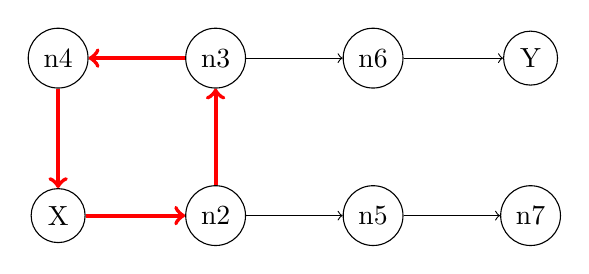
\begin{tikzpicture}
        \node[circle, draw] (n1) at (0,0) {X};
        \node[circle, draw] (n2) at (2,0) {n2};
        \node[circle, draw] (n3) at (2,2) {n3};
        \node[circle, draw] (n4) at (0,2) {n4};
        \node[circle, draw] (n5) at (4,0) {n5};
        \node[circle, draw] (n6) at (4,2) {n6};
        \node[circle, draw] (n7) at (6,0) {n7};
        \node[circle, draw] (n8) at (6,2) {Y};

        \draw[->, red, line width=1.5pt] (n1) -- (n2);
        \draw[->, red, line width=1.5pt] (n2) -- (n3);
        \draw[->, red, line width=1.5pt] (n3) -- (n4);
        \draw[->, red, line width=1.5pt] (n4) -- (n1);
        \draw[->] (n2) -- (n5);
        \draw[->] (n3) -- (n6);
        \draw[->] (n5) -- (n7);
        \draw[->] (n6) -- (n8);
    \end{tikzpicture}
    \caption{Ein zyklischer Graph}
    \label{zyklgraph}
\end{figure}

Im Kontext des Testentwurfs sind Kreise besonders interessant, da diese für einen potenziell unendlich großen Testraum sorgen.
In einem azyklischen gerichteten Graphen, also einem gerichteten Graphen, der keinen Kreis besitzt, ist die Menge aller möglichen Pfade endlich.
Bei einem Graphen mit Zyklen ist die Menge aller möglichen Pfade unendlich.
Dies folgt aus der Tatsache, dass jeder Pfad, der den Kreis beinhaltet, diesen Kreis ein weiteres Mal ablaufen kann und somit stets ein neuer Pfad generiert wird.

\newpage
  \section{GraphQL}
\label{graphql}

GraphQL~\cite{graphqlspecification} ist eine Open-Source Query-Language (Abfragesprache) und Laufzeitumgebung die von Facebook entwickelt wurde\cite[vgl. Introduction]{graphqlspecification}.
Die Besonderheiten von GraphQL sind, dass man mit nur einer einzelnen Anfrage mehrere Ressourcen gleichzeitig abfragen kann \cite[vgl. No More Over- and Underfetching]{howtographql} und die
Daten in einem Schema durch einen Typgraphen definiert sind~\cite[vgl. Benefits of a Schema \& Type System]{howtographql}.
So lässt sich die Effizienz stark erhöhen, indem weniger Anfragen gestellt werden die zeitgleich eine höhere Informationsdichte haben.
GraphQL erleichtert außerdem die Kommunikation von Schnittstellen, indem die gewünschten Felder schon in der Query definiert werden
und direkt den erwarteten Datentyp zusichern.
Hier liegt auch der große Vorteil im Vergleich zum direkten technologischen Konkurenten REST API \cite[vgl. Welche REST-Einschränkungen versucht GraphQL zu überwinden?]{awsrestgraphql}.
Bei REST-APIs sind nämlich für verschiedene Ressourcen auch jeweils eine eigene Anfrage nötig \cite[vgl. No More Over- and Underfetching]{howtographql} und die Typsicherheit ist nicht so stark gegeben
wie bei GraphQL-APIs~\cite[vgl. Zusammenfassung der Unterschiede: REST vs. GraphQL]{awsrestgraphql}.
Diese beiden großen Vorteile sorgen dafür, dass GraphQL an Popularität gewinnt und zunehmend eingesetzt wird~\cite[vgl. Continued growth and the road ahead]{graphql-growing-report}.
GraphQL ist eine Abfragesprache und Spezifikation, dies bedeutet, dass GraphQL selbst keine konkrete Implementierung für
eine Schnittstelle ist.
Implementierungen von der GraphQL-Spezifikation sind in GraphQL-Servern umgesetzt die in verschiedenen Programmiersprachen existieren.
Eine umfassende Auswahl verschiedenster Implementierungen findet sich in \cite{gqlimplementation}.
Besonderer Beliebtheit erfreuen sich ApolloServer~\cite{apolloqgl}, Express GraphQL~\cite{expressgql} und HyGraph \cite{hygql}.
Da jedoch alle Server die GraphQL-Spezifikation umsetzen müssen und unsere Tests aus GraphQL Anfragen bestehen, ist es für uns
irrelevant welche konkrete GraphQL Serverimplementierung das zu testende System verwendet.
Im Kontext dieser Arbeit ist ein tiefgreifendes, technologisches Verständniss von GraphQL essenziell, deshalb wird hier
eine tiefgreifende Erklärung von GraphQL folgen.

\subsection{Schema \& Typen}
\label{schematypes}

Grundlage einer jeden GraphQL-API ist ein GraphQL-Schema.~\cite[vgl. Core Concepts]{graphqlspecification}
Das Schema definiert exakt, wie die Daten in der API aufgebaut sind und welche Informationen exisitieren \cite[vgl. 3.2 Schema]{graphqlspecification}.
Ein GraphQL-Schema ist eine Sammlung von einzigartigen Typen und definiert die Einstiegspunkte der API.
Es gibt drei Einstiegspunkte, die $query$ zum Daten abfragen, $mutation$ zum Daten verändern und $subscription$ um über Datenänderungen informiert zu werden \cite[vgl. 3.2.1 Root Operation Types]{graphqlspecification}
$Query$ ist dabei als einziger verpflichtend, die anderen sind optional. \cite[vgl. 3.2.1]{graphqlspecification}
Die drei Einstiegspunkte sind als Typen definiert.
Ein Typ ist die fundamentale Einheit eines jeden GraphQL Schemas. \cite[vgl. 3.4 Types]{graphqlspecification}.
\newpage
Es gibt 6 verschiedene Typdefinitionen, diese sind:

\newcolumntype{C}{>{\Centering\arraybackslash}X}
\begin{center}
    \begin{table}[!ht]
        \begin{tabularx}{\textwidth}{|C|C|}
            \hline
            \textbf{ Typ } & \textbf{ Beschreibung} \\
            \hline
            \textbf{ ScalarTypeDefinition } & Primitive Datentypen die keine Verbindungen zu anderen Typen haben dürfen. (Strings, Integer, \ldots) \\
            \hline
            \textbf{ ObjectTypeDefinition  } & Komplexere Datentypen die Verbindungen untereinander haben und in Feldern ihre Verbindungen definieren \\
            \hline
            \textbf{ InterfaceTypeDefinition } & Ein abstrakter Datentyp der die Struktur für andere Typen vorgibt \\
            \hline
            \textbf{ UnionTypeDefinition } & Ein Typ der die Vereinigung verschiedener Typen ist \\
            \hline
            \textbf{ EnumTypeDefinition } & Ein Typ der nur eine feste Anzahl an vorher festgelegten Werten hat \\
            \hline
            \textbf{ InputObjectTypeDefinition } & Zusammensetzung von ScalarTypes um komplexere Eingabeargumente zu bilden  \\
            \hline
        \end{tabularx}
        \caption{GraphQL Typen\cite[vgl. 3.4 Types]{graphqlspecification}}
    \end{table}
\end{center}

Ein Typ hat einen einzigartigen Namen und definiert alle Informationen über sich, hierbei wird für jede Information ein Feld angelegt.
Das Feld setzt dann wieder jeweils einen Typen um (InputObjectTypeDefinition ist dabei ausgeschlossen).
Ein sehr einfaches Schema wäre zum Beispiel die Beziehung zwischen Büchern und Autoren.
Ein Buch hat einen Titel und einen Author.
Ein Author hat einen Namen und ein Geburtsdatum.
Zugehöriges Schema für dieses Beispiel sähe wie folgt aus:

\begin{figure}[htb]
    \begin{center}
        \begin{lstlisting}[language=GraphQL]
        type Buch {
            title: String
            author: Autor
        }
        type Autor{
            name: String
            geburtsdatum: Date
        }
        \end{lstlisting}
    \end{center}
    \caption{minimales Schema mit zwei Types}
    \label{buchauthorschema}
\end{figure}

Es lässt sich also festhalten, dass ein GraphQL-Typ immer als ein Tupel \verb+(Name, Felder)+ definiert wird wobei
die Felder eine Liste an Tupeln \verb+(Feldname, Feldtyp, Datentyp)+ sind.~\cite[vgl. 3.6 Objects]{graphqlspecification}
\newpage
Hierbei gelten folgende Einschränkungen für die Elemente des Tupels:

\begin{center}
    \begin{description}
        \item[Feldname] ein eindeutiger Feldbezeichner
        \item[Feldtyp] gibt Einschänkungen vor, z.B. nicht Null (durch \verb+!+), Listentyp (durch \verb+[]+) etc.
        \item[Datentyp] der explizite Typ den das Feld hat, kann Standarddatentyp oder anders definierter Type sein
    \end{description}
\end{center}

\subsection{Query}

Da der Query-Type der Einstiegspunkt in alle Abfragen ist, welche es später zu testen gilt, soll dieser hier nocheinmal nähere Betrachtung finden.
Sämtliche valide Abfragen beginnen im Query-Type.
Abfragen können mit und ohne Eingabeparameter angegeben werden.
Informationen darüber finden sich im Schema.
Die definierten Anfragen haben, wie jeder Typ, einen eindeutigen Bezeichner, welcher dann auch in der zustellenden Abfrage
benutzt wird.
Die Felder der Antwort hängen hierbei vom Feldtypen ab.
Ist das Ergebnis der Query-Definition ein ScalarType, so wird es direkt ausgegeben.
Ist es ein anderer definierter Typ, so müss näher bestimmt werden welche Felder erwartet werden, dabei muss die Abfrage stets mindestens ein ScalarType enthalten.
Nutzen wir das Beispiel der Bücher \& Autoren weiter, könnte man wie folgt einen Query-Type definieren:

\begin{figure}[htb]
    \begin{center}
        \begin{lstlisting}[language=GraphQL]
        type Query{
            # liste aller bücher
            getBooks: [Book]
            # ein zufälliges buch
            getBook: Book
            # author zum jeweiligen Buch
            getBookByTitle(String title): Author
        }
        \end{lstlisting}
    \end{center}
    \caption{Query Type für Buch und Autor}
    \label{minimalquerytype}
\end{figure}

Eine solche API wäre in der Lage, 3 verschiedene Anfragen zu beantworten.
Man muss beachten, dass die Anfrage \verb+getBookByTitle("Beispieltitel"){ author }+ zwingend einen Scalaren Typen aus dem Typ Autor ausweisen muss.
Die Anfrage wäre somit erst in dieser Form valide: \verb+getBookByTitle("Beispieltitel"){ author{ name } }+

\subsection{Resolver}
\label{resolver}

Bisher beschäftigen wir uns vorrangig mit der Strukturierung und Typisierung von GraphQL und den Daten die durch
das GraphQL Schema dargestellt werden.
Ein wichtiger Baustein fehlt aber noch.
Woher kommen die Daten?
Wie werden Eingabedaten behandelt?
Diese Fragen werden durch die Resolver beantwortet.
Ein Resolver ist in GraphQL eine Funktion die zuständig für die Datenabfragen und Strukturierung ist \cite[vgl.]{apolloqgl}.
Im Schema haben wir bisher definiert in welcher Art und Weise wir die Daten haben wollen, der Resolver ist nun dafür zuständig,
diese Daten im definierten Format zur Verfügung zu stellen.
Die Resolver sind nicht, wie alle vorher benannten Teil von GraphQL offen einsehbar, sondern sind Funktionen einer Programmiersprache.
Sie setzen die Schnittstellenprogrammierung wie in Kapitel~\ref{api} angesprochen um.
Für jeden Typ im Schema, muss ein Resolver implementiert werden, dies umfasst insbesondere die Query, Mutation und Subscription Typen aber auch
alle selbstdefinierten Typen \cite[vgl.]{apolloqgl}.
Die konkrete Implementierung der Resolver hängt von verschiedenen Dingen ab, insbesondere jedoch welchen GraphQL-Server man nutzt und welche Programmiersprache verwandt wird.
Ein beispielhafter Resolver für die Query eines Buches anhand seines Titels mit ApolloServer in Javascript könnte folgende minimale Syntax haben:

\begin{figure}[htb]
    \begin{verbatim}
    const resolvers = {
        Query: {
            book: (parent, args, context, info) => {
                return getBookByID(args.id);
            },
        },
    };
    \end{verbatim}
    \caption{ein einfacher Resolver}
    \label{simpleresolver}
\end{figure}

Wobei zu beachten ist, dass alle Argumente die mitgegeben werden im \verb+args+ Argument gespeichert sind.
Die Funktion $getBookByID$ gibt ein, dem Schema entsprechendes, Json-Objekt zurück.
Da die Resolver konkrete Implementierungen außerhalb von GraphQL sind und die einzelnen Resolver untereinander aufrufen können, bedarf es hier
einer Reihe an Tests da dieser Code Fehlerhaft sein kann.
Ein Klassiker für GraphQL ist es, einzelne Attribute in einem Resolver zu vergessen.
Ein Entwickler sollte für jeden Resolver, der eine Funktion darstellt, einen beziehungsweise mehrere Tests zur Verfügung stellen.
Da sich die einzelnen Resolver aber auch untereinander aufrufen können, kann sich ein teils riesiger Testraum ergeben.
Hierzu mehr in Kapitel~\ref{abfrgraph}
Um sicherzustellen, dass der Kombinationsaufruf der Resolver fehlerfrei ist, wird im Folgenden eine Methode entwickelt die gewährleistet,
dass die möglichen Kombinationen ausreichend durch Tests abgedeckt sind und so die Qualität und Zuverlässigkeit von GraphQL-APIs erhöht wird.

  \section{Zusammenhang Graphentheorie und GraphQL}

Nun, da wir ein grundlegendes Wissen über Graphentheorie und GraphQL erlangt haben, müssen wir noch zeigen,
dass Graphentheorie auch anwendbar ist auf GraphQL. Ohne diese Verknüpfung könnten wir uns nicht sicher sein,
dass die zukünftig vorgestellten Algorithmen ausführbar sind für eine GraphQL-API.

\subsection{Typen als Knoten}

Wie in $4.2.1$ schon gezeigt, ermöglicht GraphQL das Erstellen von eigenen Typen.
Diese Typen repräsentieren einzelne Datenobjekte.
Somit liegt es nahe, dass die einzelnen Typen als Knoten eines Graphens repräsentiert werden können.
Bleiben wir bei vorigem Beispiel, so definieren wir einen Typen $Book$:

\begin{figure}[ht]
    \centering
    \begin{minipage}[b]{0.4\textwidth}
        \begin{verbatim}
        type Book {
            id: Int
            title: String
        }
        \end{verbatim}
    \end{minipage}
    \hfill
    \begin{minipage}[b]{0.4\textwidth}
        \centering
        \includegraphics[width=\textwidth,height=\textheight,keepaspectratio]{img/book}
        \caption{Book als Knoten}
        \label{fig:mein_bild}
    \end{minipage}
\end{figure}

\subsection{Felder als Kanten}

Der eben definierte Typ Book besitzt aktuell nur zwei Felder, id und title.
Beides sind Skalare-Datentypen und bilden somit keine ausgehenden Kanten, denn Kanten symbolisieren Beziehungen zwischen Objekten.
Wir können einen Graphen mit $G$ = $(V,E)$ wobei $E =\emptyset$ definieren.
Allerdings wäre dies sehr restriktiv da wir überhaupt keine Verbindungen haben würden und viele Vorteile von GraphQL würden wegfallen.
Es ist aber auch möglich, dass ein Type ein Feld definiert das nicht vom Skalaren Datentyp ist.
So können wir das Buch um einen Typen $Author$ erweitern wobei der Author gleich definiert wird wie in $4.2.1$.
Diese Typdefinitionen führen dann zu diesem Graphen:

\begin{center}
    \includegraphics[width=\textwidth,height=\textheight,keepaspectratio]{img/book-author}
\end{center}

Wir nutzen also die Typdefinitionen aus um die Beziehungen zwischen einzelnen Objekten zu bekommen.
Hierbei wird ein Typ dann mit einem anderen Typen verbunden, wenn dieser als Feld im Ursprungstyp vorkommt.
Man muss hierbei klar beachten, dass dies eine gerichtete Beziehung ist.
Eben erstellte Beziehung definiert nur, dass ein Book das Feld Author hat. Wir können nach aktuellem Stand nicht
die Bücher eines Autoren herausfinden da wir diese Kante nicht deklariert haben.
Dies ist allerdings möglich. Definieren wir den Author dann also wie folgt:

\begin{verbatim}
    type Book {
        id: Int
        title: String
        author: Author
    }
    type Author {
        id: Int
        name: String
        written: [Books!]
    }
\end{verbatim}

so ergibt sich folgender, zyklischer Graph:

\begin{center}
    \includegraphics[width=\textwidth,height=\textheight,keepaspectratio]{img/book-author-circle}
\end{center}

\subsection{der komplette Graph}

Wir wissen nun also wie ein GraphQL-Schema einen Graphen repräsentiert und können Algorithmen die auf Graphen funktionieren auch
auf einem GraphQL-Schema anwenden.
Abschließend zu diesem Kapitel sei gesagt, dass es in GraphQL allerdings nicht möglich ist, jeden einzelnen Knoten direkt
abzufragen.
Dies hängt stets von der Definition des Query/Mutation-Types ab, denn alle eingehenden Anfragen müssen vom Query-Type bzw. alle
eingehenden Veränderungen müssen über den Mutation-Type ablaufen.
Der Einfachheit halber werden wir uns jetzt erstmal dem Query-Type widmen.
Jede Anfrage die in GraphQL getätigt werden kann, hat ihren Ursprung im Query-Type.
Somit folgt auch, dass alle Routen stets im Query-Type entspringen müssen.
Dies bedeutet, dass nur Knoten mit Erreichbarkeit vom Query-Type überhaupt abgefragt werden können.
In diesem Beispiel:

\begin{figure}[ht]
    \centering
    \begin{minipage}[b]{0.4\textwidth}
        \begin{verbatim}
    type Query {
        book: Book
        author: Author
    }

    type Book {
        id: Int
        title: String
        author: Author
    }
        \end{verbatim}
    \end{minipage}
    \hfill
    \begin{minipage}[b]{0.4\textwidth}
        \begin{verbatim}
    type Author {
        id: Int
        name: String
        written: [Books!]
    }

    type Publisher {
        name: String
        published:  [Book]
    }
        \end{verbatim}
    \end{minipage}
\end{figure}


wäre es nicht möglich einen Knoten des Publishers abzufragen da dieser Knoten nicht erreichbar ist vom Query-Type.

  \newpage
\section{Testen}
\label{test}

Indem technische Geräte und somit auch Software im umfangreichen Maßstab Einzug nehmen in nahezu alle Bereiche des
Lebens, ist es wichtig, die Sicherheit, Qualität und Zuverlässigkeit von Software sicherzustellen~\cite[vgl. Introduction]{software-testing}.
Um dies sicherzustellen, sind systematische Tests von Software nötig.
Dabei ist das Ziel, dass die Software bestimmten Anforderungen und Spezifikationen entspricht.
Hierbei werden diverse Techniken und Ansätze verfolgt, die im Folgenden kurz vorgestellt werden.

\subsection{Sichtweisen auf Testsysteme}

Es gibt verschiedene Sichtweisen auf das zu testende System.
Die Sichtweisen können intern oder extern bestimmt sein.
So sind Faktoren wie möglicher Zugriff auf Quellcode oder Architekturdetails des Systems essenziell wichtig, um zu entscheiden, welche Art von Tests angewandt werden sollen.
Es gibt zwei generelle Sichtweisen und eine Mischform.
Das zu testende System wird als Box betrachtet.
Diese Box kann aus verschiedenen Sichten gesehen werden, die im Folgenden näher erläutert werden.
Die Ansätze unterscheiden sich vor allem in den zur Verfügung stehenden Informationen über das System.

\subsubsection{White-Box Testing}

Im White-Box Testing stehen alle Informationen über das System zur Verfügung~\cite[vgl. 1.4.2 Code-Based Testing]{software-testing-craftmans}.
Der Tester hat Zugriff auf Code, Architekturdetails und besitzt Kenntnisse über alle möglichen Details des Systems~\cite[vgl. 1.4.2 Code-Based Testing]{software-testing-craftmans}.
Somit kann der Tester auf alle möglichen Informationen über das System zugreifen und damit seine Tests generieren.
Die erstellten Tests fundieren dann auf einem soliden Niveau, das begründet wird durch das Domänenwissen über das System.
Verschiedene Techniken zur Analyse des Domänenwissens wurden entwickelt, um die Informationen für die Testentwicklung zu nutzen.
In Kapitel~\ref{graphueberdeckung} wird eine dieser Techniken näher untersuchen.

\subsubsection{Black-Box Testing}

Im Black-Box Testing hat der Tester keinen Zugriff auf interne Funktionsweisen der Software.
Schwerpunkt des Testens ist es, dass die Software das tut, was in den Anforderungen gefordert wird~\cite[vgl. Specification-Based Testing]{software-testing-craftmans}.
Da der Quellcode nicht einsehbar ist, muss man sich darauf verlassen, dass die Anforderungen treffend formuliert wurden~\cite[vgl.]{testmanagment}.
Das Black-Box Testing hat einen methodischen Bezug zu Property-based Testing~\cite{property-based-testing}.

\subsubsection{Grey-Box Testing}

Das Grey-Box Testing ist eine Mischform von White-Box und Black-Box Tests~\cite[vgl.]{testmanagment}.
Es sind in dieser Sicht Teile der Software bekannt, aber man hat keinen umfassenden Einblick wie im White-Box Testing.
Es werden sowohl funktionale als auch strukturelle Testansätze verfolgt, je nachdem, wie viel Informationen über das System tatsächlich
verfügbar sind~\cite[vgl.]{graybox}.
Das System wird aus der Sicht des Endbenutzers getestet~\cite[vgl.]{testmanagment}, jedoch mit zusätzlichem Wissen über Teile des internen Aufbaus.

\subsection{Arten von Tests}

Neben verschiedenen Transparenzen auf dem zu testenden System gibt es verschiedene Granularitätsebenen der Tests.
Die Tests können abgeleitet werden von Anforderungen, Spezifikationen, Designartifikaten und dem Programmcode~\cite[vgl. 1.1.1 Testing Levels Based on Software Activity]{software-testing}.
Dabei können verschiedene Level an Tests definiert werden.
Die Level sind eng verbunden mit den Entwicklungsaktivitäten einer Software~\cite[vgl. 1.1.1]{software-testing}.

\begin{figure}[h!]
    \centering
    \includegraphics[width=\textwidth,height=\textheight,keepaspectratio]{img/vmodell}
    \caption{Softwareentwicklung und Test-Levels im V-Modell \cite[vgl. Figure 1.2]{software-testing}}
    \label{vmodelltest}
\end{figure}

Die verschiedenen Testebenen sollen schon im Designprozess beachtet werden, denn die Formulierung von Tests kann dabei helfen, Designfehler zu finden,
noch bevor die Software entwickelt wird~\cite[vgl. 1.1.1]{software-testing-ana}.
Die verschiedenen Ebenen der Tests spiegeln auch verschiedene Systemsichten in den Tests.
In Abbildung~\ref{vmodelltest} sind im V-Modell die verschiedenen Schritte der Softwareentwicklung abgebildet.
Dazu passend findet sich im Folgenden die Erklärung der einzelnen Ebenen.

\newpage
\begin{figure}[h!]
    \begin{description}
        \item[Akeptanz-Test] - Betrachten der Software hinsichtlich der Anforderungen
        \item[System-Test] - Betrachten der Software hinsichtlich der Architektur
        \item[Integrations-Test] - Betrachten der Software hinsichtlich der Teilsysteme
        \item[Modul-Test] - Betrachten der Software hinsichtlich detailliertem Design
        \item[Unit-Test] - Betrachten der Software hinsichtlich korrekter Implementierung
    \end{description}\cite[vgl. 1.1.1]{software-testing}
\end{figure}

Im Folgenden wird jede einzelne Testebene präziser betrachtet.
Die Reihenfolge der Betrachtung ist dabei von feingranular zu grobgranular.

\subsubsection{Unit-Tests}

Als feingranularste Testebene ist das Ziel des Unit-Tests, den entwickelten Code zu testen.
Eine einzelne $Unit$ ist in Objekt-Orientierter Programmierung eine Funktion oder Methode~\cite[vgl. Unit Testing]{software-testing-craftmans}.
Der einzelne Unit-Test konzentriert sich dabei auf eine Funktion oder Methode.

\begin{figure}[h!]
    \begin{lstlisting}[language=Python]
        def add(a, b):
            return a + b
    \end{lstlisting}
    \caption{Eine einfache Python-Funktion}
    \label{unitfkt}
\end{figure}

\begin{figure}[h!]
    \begin{lstlisting}[language=Python]
    def test_add_positive():
        self.assertEqual(add(3, 5), 8)

    def test_add_negative():
        self.assertEqual(add(-3, -5), -8)

    def test_add_mixed():
        self.assertEqual(add(5, -3), 2)
    \end{lstlisting}
    \caption{Drei Unit-Tests für die add-Funktion}
    \label{unitfkttest}
\end{figure}

Er prüft, ob die gegebene Einheit bei bekannten Eingaben die erwartete Ausgabe liefert.
Für diese Tests werden häufig Testframeworks genutzt, die bei der Entwicklung und Ausführung der Tests helfen~\cite{software-testing}.
In Abbildung~\ref{unitfkt} wurde eine Funktion definiert und in Abbildung~\ref{unitfkttest} sind drei Unit-Tests mit PyTest~\cite{pytest} definiert.
Die Tests führen verschiedene Methoden aus und prüfen, ob das Ergebnis mit der Erwartung übereinstimmt.
Das $assertEqual$ übernimmt dabei die Auswertung.

\subsubsection{Modul-Test}

Eine Granularitätsebene höher ist der Modul-Test.
Ein Modul ist eine Sammlung von Units~\cite[vgl. S. 6]{software-testing}.
Ziel ist es, die Interoperabilität der einzelnen Units in einem Modul sicherzustellen~\cite[vgl. S. 6]{software-testing}.

\begin{figure}[h!]
    \begin{lstlisting}[language=Python]
        def add(a, b):
            return a + b
        def sub(a, b):
            return a - b
        def mul(a, b):
            return a * b
        def quo(a, b):
            return a / b
    \end{lstlisting}
    \caption{Ein Python Rechenmodul}
    \label{modul}
\end{figure}

In Abbildung~\ref{modul} ist ein Rechenmodul definiert.
Dieses wird getestet, indem verschiedene Funktionen miteinander kombiniert werden und dann geprüft wird, ob Erwartung und Ergebnis übereinstimmen.
Ein Modul-Test für das Modul aus Abbildung~\ref{modul} ist in Abbildung~\ref{modultest} definiert.

\begin{figure}[h!]
    \begin{lstlisting}[language=Python]
    def test_rechenmodul():
        testResult = (mul(add(2,3), sub(3,2)))
        self.assertEqual(testResult, 5)
    \end{lstlisting}
    \caption{Ein Modul-Test}
    \label{modultest}
\end{figure}

Es ist anzumerken, dass die Interoperabilität im Modul-Test nur innerhalb eines Moduls getestet wird~\cite[vgl. S. 6]{software-testing}.

\subsubsection{Integrations-Test}

Die Integrations-Tests übernehmen das Testen von Interoperabilität zwischen verschiedenen Modulen~\cite[vgl. S. 7]{software-testing}.
Es wird davon ausgegangen, dass die einzelnen Module zuvor korrekt getestet worden sind und die einzelnen Module korrekt arbeiten~\cite[vgl. S. 7]{software-testing}.
Testobjekte sind die Schnittstellen der einzelnen Module und somit auch die Kommunikation zwischen den Modulen.

\begin{figure}[h!]
    \begin{lstlisting}[language=Python]
def newUser(name, gb, email):
    pw = generateRandomPw()
    return new User(name, gb, email, pw)
    \end{lstlisting}
    \caption{Modul 1}
    \label{modul1}
\end{figure}

\begin{figure}[h!]
    \begin{lstlisting}[language=Python]
def saveUser(User user):
    db.save(user)
def getUser(name):
    db.findUser(name)
    \end{lstlisting}
    \caption{Modul 2}
    \label{modul2}
\end{figure}

In Abbildung~\ref{modul1} ist ein Modul definiert, das einen neuen Nutzer erstellen kann.
Abbildung~\ref{modul2} definiert ein Modul, das Nutzer speichern und finden kann.
Ein Integrations-Test beider Module sollte testen, ob ein neu angelegter Nutzer ordentlich gespeichert wird und ob die dabei zugewiesenen Daten auch korrekt bleiben.
In Abbildung~\ref{integtest} ist ein solcher Integrations-Test zu finden.

\begin{figure}[h!]
    \begin{lstlisting}[language=Python]
def testAddNewUserAndSaveUserAndGetUser():
        user = newUser("Peter", "01.04.1980", "p@test.de")
        saveUser(user)
        self.assertEqual(getUser("Peter"), user)
    \end{lstlisting}
    \caption{Integrations-Test zwischen Modul 1 und Modul 2}
    \label{integtest}
\end{figure}

Im Kontext dieser Arbeit gilt es zu untersuchen, wie Integrations-Tests automatisiert für GraphQL erstellt werden können.
Hinter jedem verschiedenen Typen von GraphQL steckt ein Resolver, welcher als ein eigenes Modul gesehen werden kann.
Die Interoperabilität dieser Module gilt es im Folgenden automatisiert zu testen.

\subsubsection{System-Test}

Um zu testen, ob nicht nur einzelne Teile des Systems gut miteinander funktionieren, sondern auch das ganze System als
Solches, werden die System-Tests genutzt~\cite[vgl. S. 6]{software-testing}.
Die Tests werden auf Grundlage der Spezifikation des Systems erstellt.
Es wird davon ausgegangen, dass die einzelnen Module hier wie erwartet funktionieren.
Im Vordergrund dieser Testebene steht, dass die Software die Spezifikation, also die Erwartungen an sich, erfüllt.

\subsubsection{Akzeptanz-Test}

Die finale Ebene des Testprozesses ist der Akzeptanz-Test.
Auf dieser Ebene wird die Software aus Sicht des Endnutzers geprüft.
Dieser ist oft auch Teil dieses Prozesses~\cite[vgl. S.6]{software-testing}.
Ziel ist es, zu verifizieren, dass die Analyse und Umsetzung des Problems erfolgreich ist und der Nutzer mit der entwickelten Lösung
zufrieden ist~\cite[vgl. S.6]{software-testing}.

\subsection{Testabdeckung}
\label{abdeck}

Bisher ungeklärt ist, wann ausreichend getestet wurde und ob überhaupt genügend getestet werden kann.
Hierzu werden die formalen Abdeckungskriterien eingeführt, wie sie in~\cite{software-testing} definiert sind.
Mithilfe dieser Abdeckungskriterien wird es möglich, sinnvolle Testfälle zu entwickeln und zu entscheiden, wann ausreichend getestet wurde.
Die Notwendigkeiten für solche Abdeckungskriterien zeigt sich schnell.
Ein Ausprobieren aller Kombinationen ist in der heutigen Zeit unmöglich.
Als Beispiel sei hier eine simple Addition von 2 64-bit Integer genannt.
Für eine komplette Testung dieser Addition gibt es $2^{64}$ Kombinationen.
Mit einem 3GHz-Prozessor wäre eine vollständige Testung nach etwa 69 Tagen erledigt.
Betrachtet man einen Java-Compiler, so ist der Eingaberaum von Programmen die zum Test stehen, effektiv unendlich und somit nicht testbar~\cite[vgl. 1.3 Coverage Criteria for Testing]{software-testing}.

\subsubsection{Abdeckungskriterien}

Da ein vollständiges Testen, also ein Ausprobieren aller Möglichkeiten unmöglich ist, müssen Kriterien geschaffen werden, die eine hinreichende Testqualität zusichern.
Hierfür werden die Abdeckungskriterien eingeführt.
Diese liefern einen Ansatz, der dabei hilft, sinnvolle Tests zu entwickeln und abzuschätzen, wann ausreichend getestet wurde.
Im Folgenden werden die Abdeckungskriterien auch als Testanforderungen~\cite[vgl. 1.3 Coverage Criteria for Testing]{software-testing} gesehen.

\begin{definition}
    Eine Testanforderung ist ein spezifisches Element eines Softwareartifkates das einen Testfall erfüllen muss~\cite[Def. 1.20]{software-testing}.
    \label{tr}
\end{definition}

Dabei ist ein Abdeckungskriterium erfüllt, wenn alle seine Testanforderungen erfüllt sind.

\begin{definition}
    Ein Abdeckungskriterium ist eine Regel oder eine Sammlung von Regeln, die Testanforderungen an eine Menge von Testfällen stellen~\cite[Def. 1.21]{software-testing}.
\end{definition}

Um eine Aussage darüber zu machen, wie gut eine Menge an Tests das Abdeckungskriterium umsetzt, wird die Abdeckung eingeführt.
Einerseits ist es manchmal sehr schwierig ein Abdeckungskriterium vollständig zu erreichen, andererseits kann dann gemessen werden, ob das Kriterium erfüllt wurde~\cite[vgl. S. 18]{software-testing}.
Durch die Definition~\ref{abd} wird messbar, wie gut eine Menge an Tests das Abdeckungskriterium umsetzt und ob das Kriterium erfüllt ist.

\begin{definition}
    Gegeben sei eine Menge an Testanforderungen $TR$ für ein Abdeckungskriterium $C$. 
    Eine Menge an Testfällen $T$ erfüllt $C$ wenn gilt, 
    dass für jede Testanforderung mindestens ein Test existiert der diese Testanforderung erfüllt~\cite[vgl. Def. 1.22]{software-testing}.
    \label{abd}
\end{definition}

Es gibt diverse Abdeckungskriterien, die auf verschiedenen Annahmen beruhen.
Ist das Ziel, dass alle Entscheidungen in einem Programm abgedeckt sein sollen (Branch-Coverage), so führt jede Entscheidung zu zwei
Testanforderungen, eine Anforderung für den positiven und eine für den negativen Entscheidungsfall~\cite[vgl. S. 17]{software-testing}.
Soll jede Methode mindestens einmal aufgerufen werden (Call-Coverage), so führt jede Methode zu einer Testanforderung, um diese Methode abzudecken~\cite[vgl. S. 17]{software-testing}.
Im folgenden Kapitel~\ref{graphueberdeckung} werden Abdeckungskriterien speziell für Graphen eingeführt.
  \chapter{Graphcoverage}

Wie zuvor gesehen, existieren verschiedene Coverage-Kriterien um Testabdeckung zu prüfen.
Graphcoverage ist hierbei eine Herangehensweise um graphenbasierte Datenstrukturen zu überdecken.
Graphen können nämlich ähnliche Probleme aufweisen wie vorheriges Beispiel der Addition.
Die Addition zweier 64-bit Integer ist wenigstens endlich, Graphenstrukturen haben sogar unter Umständen unendliche Testräume.
Umso wichtiger ist es hier, dass Überdeckungskriterien formuliert werden können, die diesen möglicherweise unendlichen Suchraum
stark verkleinern und dennoch eine ausreichende Testung ermöglichen.
Da wir vorher ergründet haben, dass GraphQL sich als gerichteten Graph darstellen lässt, können wir nun die Graphcoverage nutzen, um Tests mithilfe der Grapcoverage zu erstellen.
Wie genau die Coverage erstellt wird und daraus Tests resultieren, werden im folgenden geklärt.
Gerichtete Graphen sind die Grundlage für viele Coverage-kriterien, wobei die Grundidee hierbei ist,
Sachverhalte als Graphen zu modellieren und dann eine ausreichende Überdeckung zu finden. \cite[vgl. Software-testing S. 27 2.1]{software-testing}
In $4.1.2$ wurden gerichtete Graphen bereits eingeführt, daher können wir direkt fortfahren und verschiedene
Kriterien definieren, die einen Graphen überdecken.
Wir erklären zuerst verschiedene Techniken, die einen Graphen überdecken und erklären dann ihre Anwendung
an Beispielen.
Erst sortieren wir Graphcoverage ein im Kontext von Code-Coverage und bilden im zweiten Schritt eine Coverage für GraphQL\@.

\section{Graphcoverage allgemein}

Um Graphcoverage zu nutzen, verfeinern wir zuerst die allgemeine Definition von gerichteten Graphen.
Ein gerichteter Graph ist ein Paar $G = (V, E)$ zweier disjunkter Mengen mit $E \subseteq V^2$ wobei alle Elemente aus E gerichtete Kanten sind. [vgl. 4.1.2]
Die Definition erweitern wir nun mit:

\begin{description}
    \item[Menge N] von Knoten
    \item[Menge N_{0}] von Anfangsknoten, wobei N_{0} $\subseteq$ N
    \item[Menge N_{f}] von Endknoten, wobei N_{f} $\subseteq$ N
    \item[Menge E] von Kanten, wobei E $\subseteq$ N x N. Hierbei ist die Menge als init{x} x target{y} definiert.
\end{description}~\cite[2.1 Overview]{software-testing}

Mithilfe dieser Definition können nun zum Beispiel Kontrollflussgraphen abgebildet werden indem die Einstiegspunkte die Anfangsknoten sind und die Endknoten die Austrittspunkte.
Ein Pfad innerhalb von eben definierten Graphen, mit möglicher Länge Null, der in einem Knoten $N_{0}$ startet und in einem Knoten $N_{f}$ endet, nennt sich Testpfad \cite[vgl. S. 28]{software-testing}
Ziel ist es nun mit hilfe von Coverage-Kriterien Testpfade zu ermitteln die unser Problem ausreichend testen - was hierbei ausreichend ist, ist von Fall zu Fall unterschiedlich.

\section{Graphcoverage Kriterien}

Mithilfe voriger Definition können wir nun Coveragekriterien entwickeln, die uns Testpfade liefern, die je nach Kriterium für eine spezielle Abdeckung
des Graphens mit Test-Requirements sorgen.

\subsection{Node Coverage}

Node-Coverage ist ein Coveragekriterium, dass alle Knoten, die von $N_{0}$ erreichbar sind, in einem Graphen abdecken soll.
Definieren wir folgenden, sehr einfachen Graphen:

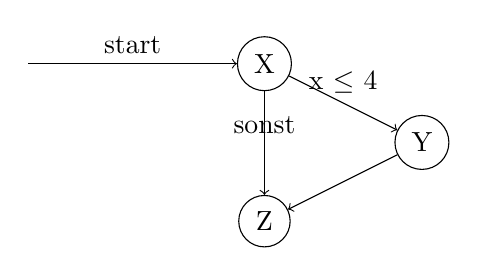
\begin{tikzpicture}
    \node[circle, draw] (n1) at (2,2) {X};
    \node[circle, draw] (n2) at (4,1) {Y};
    \node[circle, draw] (n3) at (2,0) {Z};

    \draw[->] (-1,2) -- node[above] {start} (n1);
    \draw[->] (n1) -- node[above] {x $\le$ 4} (n2);
    \draw[->] (n2) -- (n3);
    \draw[->] (n1) -- node[above] {sonst} (n3);
\end{tikzpicture}

So wäre die Node-Coverage mit einem Test einzigen Test erfüllbar.
Dieser ist der Pfad $X \rightarrow Y \rightarrow Z$.
Es ist auch denkbar, dass wir zwei Pfade oder mehr nutzen allerdings erfüllt dieser Pfad schon unser Kriterium daher geben wir uns vorerst zufrieden.
Wir sehen schnell, dass dieser Ansatz noch Lücken aufweist, da der Pfad $X \rightarrow Y \rightarrow Z$ das Kriterium erfüllt, allerdings wird eine Kante $X \rightarrow Z$ nicht im
Test berücksichtigt und kann somit ungetestet bleiben.
Wir führen also noch andere Kriterien ein, die eher geeignet wären.

\subsection{Edge-Coverage}

Edge-Coverage ist ein Coveragekriterium, dass die Kanten in einem Graphen abdecken soll.
Ziel der Edge-Coverage ist es, dass jede Kante des Graphens durch mindestens einen Test abgedeckt wird.
Um die Edge-Coverage für vorheriges Beispiel zu erreichen, benötigen wir schon zwei Routen.
Der Graph:

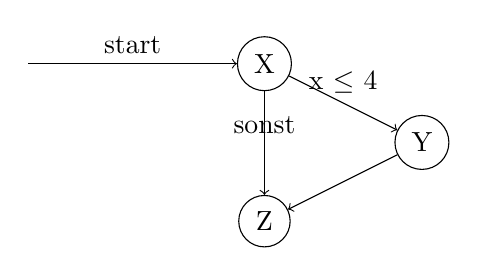
\begin{tikzpicture}
    \node[circle, draw] (n1) at (2,2) {X};
    \node[circle, draw] (n2) at (4,1) {Y};
    \node[circle, draw] (n3) at (2,0) {Z};

    \draw[->] (-1,2) -- node[above] {start} (n1);
    \draw[->] (n1) -- node[above] {x $\le$ 4} (n2);
    \draw[->] (n2) -- (n3);
    \draw[->] (n1) -- node[above] {sonst} (n3);
\end{tikzpicture}

wird über die Pfade $X \rightarrow Y \rightarrow Z$ und $X \rightarrow Z$ überdeckt.
Edge-Coverage hat allerdings auch Probleme Graphen vollständig zu überdecken.
Man nehme folgendes Beispiel:

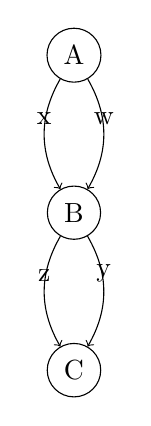
\begin{tikzpicture}
    \node[circle, draw] (a) at (4,4) {A};
    \node[circle, draw] (b) at (4,2) {B};
    \node[circle, draw] (c) at (4,0) {C};

    \draw[->, bend left=30] (a) to node[above] { w } (b);
    \draw[->, bend right=30] (a) to node[above] { x } (b);
    \draw[->, bend left=30] (b) to node[above] { y } (c);
    \draw[->, bend right=30] (b) to node[above] { z } (c);
\end{tikzpicture}

Pfade die laut Edge-Coverage ausreichen um den Graphen zu überdecken wären: \\
$ x \rightarrow z $ \\
$ w \rightarrow y $ \\
Hierbei wird allerdings außer acht gelassen, dass in $x$ auch Änderungen passieren können die Auswirkungen im Programm haben können.
So sind die Routen $ x \rightarrow y $ und $ w \rightarrow z $ in der Edge-Coverage nicht berücksichtigt.
Allerdings wären diese auch zu testen.
Wir sehen also, dass wir immer noch kein ideales Kriterium gefunden haben.


\subsection{Edge-Pair Coverage}

Das Edge-Pair Coveragekriterium ist eine Erweiterung der Edge-Coverage, indem hier auch die Beziehungen von einzelnen Kanten untereinander berücksichtigt werden um das zuvor
aufgetretene Problem zu lösen.
Nach \cite[Introduction to Software Testing]{software-testing} ist Edge-Pair Coverage: ''Alle erreichbaren Pfade von Länge bis zu 2 im Testgraphen''.
Ziel dieses Coverage-Kriteriums ist es, dass alle möglichen Kantenpaare abgedeckt sind.
Eben definiertes Beispiel hätte mit Edge-Pair Coverage eine Überdeckung mit: \\
$ x \rightarrow z $ \\
$ w \rightarrow y $ \\
$ x \rightarrow y $ \\
$ w \rightarrow z $

Dieses simple Beispiel wird durch Edge-Pair Coverage gut abgedeckt.
Edge-Pair Coverage neigt allerdings dazu, extrem große Suchräume zu erzeugen und nur Pfadkombinationen bestimmter Länge zu betrachten. \cite[vgl. S. 35]{software-testing}
Hierdurch werden bestimmte Kombinationen von Pfaden immer noch nicht berücksichtigt.

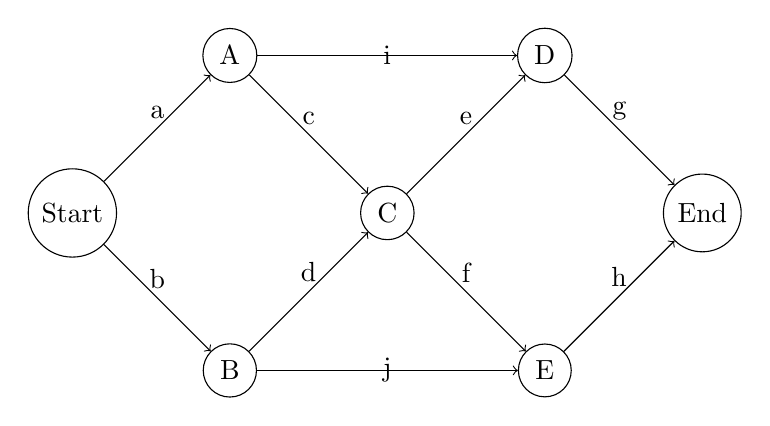
\begin{tikzpicture}
    \node[circle, draw] (start) at (0,0) {Start};
    \node[circle, draw] (a) at (2,2) {A};
    \node[circle, draw] (b) at (2,-2) {B};
    \node[circle, draw] (c) at (4,0) {C};
    \node[circle, draw] (d) at (6,2) {D};
    \node[circle, draw] (e) at (6,-2) {E};
    \node[circle, draw] (end) at (8,0) {End};

    \draw[->] (start) to node[above] { a } (a);
    \draw[->] (start) to node[above] { b } (b);
    \draw[->] (a) to node[above] { c } (c);
    \draw[->] (b) to node[above] { d } (c);
    \draw[->] (c) to node[above] { e } (d);
    \draw[->] (c) to node[above] { f } (e);
    \draw[->] (d) to node[above] { g } (end);
    \draw[->] (e) to node[above] { h } (end);
    \draw[->] (a) to node[out=30, in=150] { i } (d);
    \draw[->] (b) to node[out=-30, in=210] { j } (e);
\end{tikzpicture}

Nach der Definition von Edge-Pair Coverage ermitteln wir erstmal alle Pfadkombinationen der Länge ''bis zu 2''
Dies wären:

$Start \rightarrow A \rightarrow C$ \\
$Start \rightarrow A \rightarrow D$ \\
$Start \rightarrow B \rightarrow C$ \\
$Start \rightarrow B \rightarrow E$ \\
$A \rightarrow C \rightarrow D$ \\
$A \rightarrow C \rightarrow E$ \\
$B \rightarrow C \rightarrow D$ \\
$B \rightarrow C \rightarrow E$ \\
$A \rightarrow D \rightarrow End$ \\
$B \rightarrow E \rightarrow End$ \\
$C \rightarrow D \rightarrow End$ \\
$C \rightarrow E \rightarrow End$ \\

Hierdurch ergeben sich dann diese Testpfade:

$Start \rightarrow  A \rightarrow  C \rightarrow  D \rightarrow  End$ \\
$Start \rightarrow  A \rightarrow  C \rightarrow  E \rightarrow  End$ \\
$Start \rightarrow  B \rightarrow  C \rightarrow  D \rightarrow  End$ \\
$Start \rightarrow  B \rightarrow  C \rightarrow  E \rightarrow  End$ \\

allerdings fehlen auch hier wieder Pfade. \\
Zum Beispiel der Pfad $Start \rightarrow A \rightarrow D \rightarrow End$ fehlt.
Hierdurch bleiben wieder Teile des Graphens unüberdeckt.

\subsection{Prime-Path Coverage}

Die Prime-Path Coverage verlangt, dass jeder (Prime)Primärpfad durch mindestens einen Testpfad abgedeckt sein muss.
Ein Primärpfad ist definiert als ein einfacher Pfad, der nicht vollständig als zusammenhängender Teil in einem anderen einfachen Pfad enthalten ist. \cite[vgl. S. 35]{software-testing}
Hierbei ist ein einfacher Pfad dann  ein Pfad, in dem keine Kanten und keine Knoten wiederholt werden,
mit Ausnahme möglicherweise des ersten und letzten Knotens (wenn sie gleich sind, handelt es sich um einen Kreis).
In diesem Graphen:

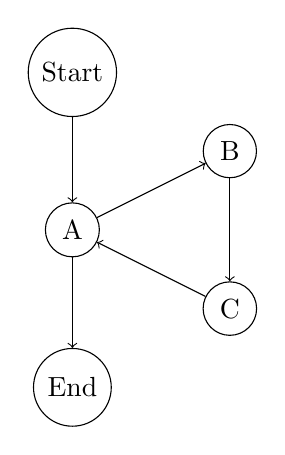
\begin{tikzpicture}
    \node[circle, draw] (start) at (4,4) {Start};
    \node[circle, draw] (a) at (4,2) {A};
    \node[circle, draw] (b) at (6,3) {B};
    \node[circle, draw] (c) at (6,1) {C};
    \node[circle, draw] (d) at (4,0) {End};


    \draw[->] (start) to node[above] { } (a);
    \draw[->] (a) to node[above] { } (b);
    \draw[->] (b) to node[above] { } (c);
    \draw[->] (a) to node[above] { } (d);
    \draw[->] (c) to node[above] { } (a);
\end{tikzpicture}

Sind dies alle Prime-Paths: \\

$ Start \rightarrow  A \rightarrow  End$ \\
$ Start \rightarrow A \rightarrow B \rightarrow C$ \\
$ A \rightarrow B \rightarrow C \rightarrow A $ \\
$ B \rightarrow C \rightarrow A \rightarrow B $ \\
$ C \rightarrow A \rightarrow B \rightarrow C $ \\
$ B \rightarrow C \rightarrow A \rightarrow End $ \\

und schon zwei Testpfade würden ausreichen um die Prime-Path Coverage zu erfüllen.
Die Testpfade die das Testrequirement erfüllen sind:

$Start \rightarrow A \rightarrow End$ \\
$Start \rightarrow A \rightarrow B \rightarrow C \rightarrow A \rightarrow B \rightarrow C \rightarrow A \rightarrow End$

\subsection{Complete-Path Coverage}

Als letztes Coveragekriterium wollen wir die Complete-Path Coverage einführen.
Ziel dieses Coveragekriteriums ist es, dass jeder mögliche Pfad mit einem Test abgedeckt werden kann.
Wir brauchen dieses Kriterium nicht ausführlich definieren, da in zyklischen Graphen eine Complete-Coverage nicht möglich ist.
Kreise in Graphen führen zu einer unendlich großen Menge an Pfaden und wir können keine unendlich große Menge behandeln.
Die Complete-Path Coverage ist sinnvoll wenn wir Kreise verbieten und der Testgraph nicht zu groß ist.
Um unsere Methode jedoch von \cite[Property-based Testing]{property-based-testing} abzugrenzen wollen wir explizit Kreise erlauben.
Ja sogar fördern um zu symbolisieren warum unsere Methode eine Verbesserung darstellt.


\subsection{abschließender Vergleich der Coverage-Kriterien}


\section{Graphcoverage für Code}

\section{Graphcoverage für GraphQL}






  \chapter{Testprozess}
\label{testentwurf}

Nachdem wir zuvor festgestellt haben, dass die PrimePfad Abdeckung potenziell das sinnvollste Abdeckungskriterium ist, wollen wir im folgenden
eine Methodik entiwckeln die es erlaubt, mithilfe dieses Abdeckunskriteriums Tests für GraphQL zu entwerfen.
Die zu entwickelnde Methodik wird in einigen Teilen stark an der Methode aus~\cite{property-based-testing} orientiert sein, dies wird
jedoch an den betreffenden Stellen kenntlich gemacht.
In diesem Kapitel wird die Methodik konzeptionell entwickelt und im folgenden Kapitel~\ref{testautomatisierung} ein Prototyp entwickelt, der
die Methodik umsetzt und validiert.
Die zu entwickelnde Methode arbeitet grob nach dem in Abbildung~\ref{methodeablauf} gezeigtem Muster.

\begin{figure}[H]
    \centering
    \includegraphics[width=0.75\textwidth,keepaspectratio]{img/fktweiseprototyp}
    \caption{Grober Ablauf des Testprozesses}
    \label{methodeablauf}
\end{figure}

Wie in Abbildung~\ref{methodeablauf} zu sehen ist der gesamte Testprozess in zwei Teile aufgeteilt.
Einerseits in den Testentwurf und andererseits in die Testausführung.
Der Testentwurf basiert auf den zuvor erarbeiteten Theorien und die Testausführung orientiert sich stark am
Property-based Testing \cite[vgl. Method]{property-based-testing}.

\section{Testentwurf}

Der erste Abschnitt des Testprozesses erarbeitet die Pfadgenerierung nach gewähltem Abdeckungskriterium.
Wie zuvor ermittelt, wird die PrimePfad Abdeckung im folgenden ermittelt.
Die Methode erlaubt allerdings auch einen Wechsel des Abdeckungskriteriums da im Endeffekt nur die Pfade für die weiteren Prozesse
genutzt werden können.
Bevor jedoch ein Abdeckungskriterium genutzt werden kann, muss das GraphQL-Schema in einen Graphen übersetzt werden.

\subsection{GraphQL-Schema in Graph abbilden}
\label{schemagraph}

Laut GraphQL-Specification~\cite{graphqlspecification} erlaubt ein GraphQL Server, dass Abfragen über die Schemastruktur des
Servers erlaubt sind \cite[vgl. 4. Introspection]{graphqlspecification}.
Mithilfe einer Introspection-Query \ref{introspection-query} lässt sich das gesamte Schema eines GraphQL-Servers abrufen.
Die Introspection-Query existiert in verschiedenen Varianten, wir nutzen hier die exakt gleiche Version wie sie auch von \cite[]{property-based-testing} genutzt wird.
Ergebnis der Introspection Query ist ein JSON-Objekt mit einer Struktur wie in Listing~\ref{introspec} gezeigt.

\begin{lstlisting}[language=json, caption={Schema-Response},captionpos=b]
    {
        "data": {
            "__schema": {
                "queryType": {},
                "mutationType": {},
                "subscriptionType": {},
                "types": [],
                "directives": []
            }
        }
    }
\end{lstlisting}
\label{introspec}

Der Eintrag $queryType$ gibt den Namen des Typens an, der Startpunkt jeder Query ist, so wie in Kapitel\ref{gqlcov} festgelegt.
Mit dem Eintrag $types$ erhalten wir eine Liste aller Typen wobei jeder Eintrag der Struktur in Listing\ref{typstrukt} entspricht.

\begin{lstlisting}[language=json, caption={Type-Field},captionpos=b]
        {
          "kind": "",
          "name": "",
          "description": "",
          "fields": [],
          "inputFields": [],
          "interfaces": [],
          "enumValues": [],
          "possibleTypes": []
        }
\end{lstlisting}
\label{typstrukt}


Um nun aus dem Schema einen Graphen zu erstellen, benötigen wir die Felder $kind$, $name$, $fields$.
$kind$ ist die Angabe, von welchem Typ das Feld ist.
Hierbei gibt es 9 Möglichkeiten, die dieses Feld annehmen kann.

\begin{itemize}
    \item \textbf{ObjectTypeDefinition (OBJECT):} Repräsentiert ein Objekt mit Feldern.
    \item \textbf{ScalarTypeDefinition (SCALAR):} Eingebaute oder benutzerdefinierte Typen wie \texttt{Int}, \texttt{Float}, \texttt{String}, \texttt{Boolean} und \texttt{ID}.
    \item \textbf{InputObjectTypeDefinition (INPUT\_OBJECT):} Erlaubt das Übergeben komplexer Objekte als Argumente.
    \item \textbf{InterfaceTypeDefinition (INTERFACE):} Repräsentiert eine Liste von Feldern, die andere Objekttypen enthalten müssen.
    \item \textbf{UnionTypeDefinition (UNION):} Kann einen von mehreren Arten von Objekttypen repräsentieren.
    \item \textbf{EnumTypeDefinition (ENUM):} Ein Skalartyp, der auf eine bestimmte Liste von Werten beschränkt ist.
    \item \textbf{ListTypeDefinition (LIST):} Repräsentiert eine Liste von Werten eines bestimmten Typs.
    \item \textbf{NonNullTypeDefinition (NON\_NULL):} Ein Modifikator, der angibt, dass der angewandte Typ nicht null sein kann.
    \item \textbf{DirectiveDefinition (DIRECTIVE):} Passt das Verhalten von Feldern oder Typen  Schema an.
\end{itemize}

Um einen Graphen aus dem Schema zu entwickeln benötigen wir nur Felder vom Typ $OBJECT$.
Die Menge aller Objekte vom Typ $OBJECT$ sind die Menge aller Knoten unseres Graphens.
Um nun die Kanten, also die Beziehungen zwischen diesen einzelnen Knoten zu bekommen müssen wir uns die Defintion
eines Typens näher ansehen.
Wie in $Type-Field$ gesehen, definiert ein Type immer ein Feld $fields$.
In diesem Feld $fields$ verbirgt sich die Informationen aller Kanten, die ausgehend von diesem Knoten sind.
Das Feld $fields$ beeinhaltet Objekte folgender Struktur:

\begin{lstlisting}[language=json, caption={Type-Field},captionpos=b]
            {
              "name": "",
              "description": "",
              "args": [],
              "type": {},
              "isDeprecated": "",
              "deprecationReason": ""
            }
\end{lstlisting}

Wobei für die Kantensuche das Feld type besonders wichtig ist.
Dieses ist wie folgt definiert:

\begin{lstlisting}[language=json, caption={Type-Field},captionpos=b]
    {
        "kind": "",
        "name": "",
        "ofType": null
    }
\end{lstlisting}

Wenn nun der Eintrag $kind$ den Wert $OBJECT$ trägt, so ist klar, dass unser hier definiertes $OBJECT$ eine Kante zum
Knoten $name$ besitzt.

\subsection{Testpfade ermitteln}
\label{testpfade}

Da wir nun einen Graphen passend zum Schema ermittelt haben, gilt es, die Testpfade zu ermitteln, welche die PrimePfad-Abdeckung erfüllen.
Hierzu nutzen wir den in~\cite[Finding Prime Test Paths]{software-testing} vorgestellten Algorithmus.
Dabei werden zuerst die einfachen Pfade ermittelt und dann gefiltert.
Dies sind Pfade ähnlich zu Definition~\ref{primepfad} mit der Lockerung, dass diese Pfade auch Teilpfad eines längeren Pfades sein können~\cite[vgl. S. 35]{software-testing}.
Der längste einfache Pfad kann maximal so lang sein wie die Anzahl der Knoten des Graphens~\cite[vgl. S.41 ]{software-testing}.
Nun wird von jedem Knoten aus expandiert und eine Liste über alle Pfade geführt.
Pfade werden nicht weiter expandiert, wenn diese einen Knoten doppelt enthalten.
Endergebnis ist dann eine Liste aller einfachen Pfade.
Filtert man die einfachen Pfade heraus, die Teil eines anderen Pfades sind erhält man nach Definition~\ref{primecov} die PrimePfad Abdeckung da
wir alle PrimePfade gefunden haben denn es gilt, dass die Menge der Primepfade eine echte Teilmenge der einfachen Pfade ist~\cite[vgl. S. 35]{software-testing}.
Mit der Einschränkung von GraphQL, dass valide Querys stets im Query-Knoten starten müssen, muss sichergestellt werden, dass die PrimePfade dort starten.
Um dies umzusetzen legen wir fest, dass der kürzeste Weg vom Query Knoten zum Startknoten des PrimePfades zu ermitteln ist und an den PrimePfad anzuhängen,
sodass aus diesem später eine valide Query generiert werden kann.

\section{Testausführung}

Die ermittelten Pfade werden nun zu validen GraphQL-Querys umgewandelt und dann ausgeführt um den Test zu validieren.
Die Pfadumwandlung in eine valide Query ist noch methodisch stark abweichend zu \cite{property-based-testing}.
Die späteren Schritte, also Test ausführen und auswerten sind methodisch gleich zu \cite{property-based-testing}.

\subsection{Pfade in Query umwandeln}
\label{pfadquery}

Einen Pfad wandeln wir in eine konkrete Query um indem wir die Typinformationen aus dem Schema nutzen.
Beginnend im Query-Knoten wird der Pfad iteriert.
Das GraphQL-Schema enthält Informationen darüber, welche Informationen nötig sind um zum nächsten adjazenten Knoten des Pfades zu kommen.
Die Informationen darüber sind im Eintrag $fields$ enthalten wie in Listing~\ref{typstrukt} gesehen.
Im $fields$ Eintrag steht dann, ob eine Kante Argumente benötigt und welcher Typ das Rückgabeobjekt ist.
Das Rückgabeobjekt des $fields$ steht dabei aber schon fest da dieser exakt gleich sein muss mit dem nächsten Knoten des Pfades.
In jedem Schritt der Query-Generierung werden stets alle Felder vom Typ $SCALAR$ hinzugefügt, damit sichergestellt werden kann, dass
der Typ alle Felder implementiert hat.
Je nach Implementierung können durch die Feldauswahl weitere Funktionen abgefragt werden, daher inkludieren wir schlichtweg alles.
Felder vom Typ $OBJECT$ werden nur zur Query hinzugefügt, wenn der Typ des $OBJECT$ dem nächsten Knoten entspricht.
Im Allgemeinen lässt sich das Verfahren in diesem Pseudocode darstellen: \\

\begin{verbatim}
    path = (A , B , ..... , Y)
    query = {}

    while path not empty:
        knoten = pfad.pop()
        ScalarFields = getScalarFields(knoten)
        query.addScalars(ScalarFields)
        edge = pfad.peek()
        args = checkForEdgeArgs(edge)
        query.addArgs(args)
    return query
\end{verbatim}

Die Argumente die in einer Query verwendet werden, sind stets nur $SCALAR$ Types und somit einfache Datentypen.
Es gibt verschiedene Arten die Argumentgeneratoren umzusetzen, vorerst werden diese jedoch methodisch exakt wie in \cite{property-based-testing} genutzt.
Dabei wird der Typ des Arguments genutzt um zufällig ein Argument des entsprechenden Typens zu generieren.
Ergebnis des Prozesses ist schließlich eine valide GraphQL-Query.
In einer konkreten Implementierung ist die Syntax von GraphQL zu beachten, diese ist einsehbar in \cite[2.3 Language Operations]{graphqlspecification}.

\subsection{Querys an SUT senden}
\label{testf}

Die generierten Querys stellen die konkreten Tests für GraphQL dar.
Um diese auszuführen, werden alle generierten Querys per \textit{HTTP-POST} an den GraphQL-Server geschickt und die Antworten
werden gespeichert, dies ist analog zu \cite{property-based-testing}.
Es ist wünschenswert, dass die generierten Querys in einem Testframework abgebildet und gespeichert werden.
Dadurch werden die Tests reproduzierbar und können später verwendet werden um etwaige Fehlerbehebungen zu verifizieren.

\subsection{Testauswertung}

Die Auswertung der Tests basiert im Grunde auf den selben Annahmen wie Sie in \cite{property-based-testing} getroffen wurden.
Dabei werden die HTTP-Codes der Antworten und die existierenden Keys in der Response überprüft.
Eine Antwort eines GraphQL-Server liefert stets einen Statuscode \textbf{200} wenn kein kritischer Fehler auftrat.
Kritische Fehler sind stets ein Statuscode \textbf{500} \cite[vgl. 7. Response]{graphqlspecification}.
Daher wird jede Antwort mit einem Code \textbf{500} als gefundenere Fehler und fehlerhafter Test betrachtet.
Eine Antwort mit einem Statuscode \textbf{200} kann jedoch auch Fehler aufweisen.
Dies wird ersichtlich durch einen zweiten Haupteintrag $errors$ in einer Antwort, ersichtlich in Listing~\ref{err}

\begin{lstlisting}[language=GraphQL, label={err}, caption={fehlerhafte Antwort}]
    {
        "data": {}
        "errors": {}
    }
\end{lstlisting}

Hierbei müssen die $errors$ jedoch manuell geprüft werden ob es sich um wirkliche Programmierfehler handelt oder gewünschtem Verhalten,
da die Zufallsargumente teilweise dafür sorgen, dass Konventionen nicht eingehalten werden können.
Die Zufallsargumente sorgen allerdings auch dafür, dass die errechnete PrimePfad Abdeckung nicht praktisch umgesetzt wird.
Sehr häufig kommt es vor, dass zufällig generierte Argumente schon in den Anfängen des Pfades nicht passend zu den unterliegenden Daten sind.
Dadurch folgt, dass ein Großteil der Testpfade die theoretisch eine gute Abdeckung aufweisen, praktisch diese Abdeckung nicht erreichen.
Um Messen zu können, ob ein Pfad seine theoretische Abdeckung auch praktisch erreicht, führen wir eine Abschätzung darüber ein.

\subsubsection{Abschätzung der Pfadlängen}
Diese Methode verbessert zwar nicht die Testergebnisse allerdings gibt Sie uns Informationen darüber wie viel von unserem Pfad in Wirklichkeit
abgedeckt wurden.
Dadurch lässt sich der Erfolg der Tests besser abschätzen da wir so messen können, ob die Querys wirklich die Funktionen ausgeführt haben.
Hierzu wird die Pfadlänge des Pfades der zur Erstellung der Query genutzt wurde als erwartete Pfadlänge angenommen.
Die Pfadlänge der Antwort wird dann als tatsächliche Pfadlänge genommen.
Der Unterschied zwischen erwarteter und tatsächlicher Pfadlänge ist dann unser Auswertungsmerkmal für diesen speziellen Test.
Die Pfadlänge der Response ist die maximale Tiefe der JSON-Response verringert um 1.

\[ \text{Tiefe des Pfades} = \text{Tiefe des JSON-Response-Objekts} - 1 \]

Demnach hätte folgende Response eine Tiefe von 2
\begin{lstlisting}[language=GraphQL, caption={vollständige Response}]
    {
        "data": {
            "book": {
                id: "1",
                title: "Moby Dick"
                publisher: {
                    id: "1",
                    name: "Testverlag"
                }
            }
        }
    }
\end{lstlisting}

Und die leere Antwort hätte eine Tiefe von 1

\begin{lstlisting}[language=GraphQL, caption={mangelhafte Response}]
    {
        "data": {
            "book": null
        }
    }
\end{lstlisting}

Obwohl eine leere Response zulässig ist und nicht auf einen Fehler hindeutet, signalisiert uns der Unterschied zwischen erwarteter und tatsächlicher Länge dann,
ob die Query tatsächlich alle Resolver ausgeführt hat oder nur einen Teil davon.
Hierdurch können wir die Tests in ihrer Qualität auswerten.
Wir können die Pfadlängen aller erwarteten Pfade addieren, das gleiche müssen wir auch mit den tatsächlichen Pfadlängen machen.
So erreichen wir zwei Zahlen und mit diesen können wir eine prozentuale Einschätzung abgeben, wieviel Prozent unserer Tests
insgesamt ausgeführt wurden.
Wir rechnen hierfür:

\[ \text{Prozent der tatsächlichen Abdeckung} = \frac{\text{tatsächliche Gesamtpfadlänge}}{\text{erwartete Gesamtpfadlänge}} * 100 \]

Wir sollten einen Wert von 100\% anstreben.
Dies würde bedeuten, dass unsere generierten Tests auch alle Funktionen getestet haben.
Andernfalls bedeutet ein Prozentsatz unter 100\% eben, dass nicht alle Funktionen tatsächlich von den Querys überdeckt wurden.

\\
\\

Abschließend wollen wir noch kurz erläutern, wie es möglich wäre, die Tatsächliche Abdeckung zu erhöhen.
Dies geschieht vor allem durch ein anpassen der Zufallsgeneratoren und die Anzahl der Querys.

\subsubsection{Zufallsgeneratoren der Argumente}
\label{zufallsgen}

Die zuvor vorgestellte Abschätzung liefert uns einen Hinweis darauf, wie gut unsere Querys tatsächlich getestet haben.
Ein Ansatz der die Querys eine bessere tatsächliche Abdeckung zu erreichen lässt ist das anpassen der Generatoren für die Argumente.
In der vorgestellten Methode in Kapitel~\ref{pfadquery} erstellen wir komplett zufällig Argumente für die Funktionen.
Dies bedeutet, dass z.B. der Type $ID$ als String gewertet wird.
Dieser Type ist in der Realität jedoch eingeschränkt und gleichzeitig sehr bedeutend, da dieser häufig als Argument angegeben wird und er eine spezielle Struktur hat.
Es hängt natürlich stark von der eigenen Implementierung der GraphQL-API ab allerdings wenn in der Implementierung
eine $ID$ definiert ist als Zahlenstring, so kann es sich durchaus lohnen, dass der Argumentgenerator für die ID auch speziell
auf Zahlenstrings angepasst wird.
Alternativ kann auch eine Liste aller existenten IDs angegeben werden und zufällig ausgewählt werden.
Die Anpassung der Argumentgeneratoren an die zugrundeliegenden Daten ist höchst spezifisch und daher kann keine allgemeine
Vorgehensweise ermittelt werden.
Ziel der Anpassung ist es, dass die Chance erhöht wird mit der Argumente zufällig generiert werden, die dann tatsächlich zu Zugrunde liegenden Daten passen.

\subsubsection{Anzahl der Querys}

Die Wahrscheinlichkeit passende Argumente zu generieren steigt außerdem mit der Anzahl an generierten Querys.
Erhöht man die Anzahl an generierten Querys pro PFad, so erhöht sich auch die Wahrscheinlichkeit, dass zumindest ein Pfad
eine gute Abdeckung erreicht.
Hierfür müssen wir die Methode aus Kapitel~\ref{pfadquery} so oft wie gewünscht wiederholen, sodass wir verschiedene Querys mit verschiedenen Argumenten erhalten.
Bei dieser Methode ist wichtig, dass sich die Argumente der Querys verändern da wir sonst einfach mehrfach die selbe Query stellen mit der
gleichen zu erwartenden Antwort.
Zusammen mit den angepassten Argumentgeneratoren kann so das zufallsbasierte Argumentgenerieren ein wenig begrenzt werden
und es ist wahrscheinlicher, dass gute Tests entstehen.

\section{Zusammenfassung der Methode}

Wir wollen im folgenden die eben vorgestellte Methode noch einmal kurz zusammenfassen damit diese übersichtlicher wird.
Unsere hier vorgestellte Methode funktioniert so wie in Abbildung~\ref{methodeablauf} gezeigt.
Wie zu sehen, ist der ganz grobe Ablauf ähnlich zum~\cite[Property-based Testing]{property-based-testing} allerdings unterscheidet sich die
Methode in einigen Teilen sehr stark vom~\cite[Property-based Testing]{property-based-testing}.
Wir fügen in unserer Methode den Schritt hinzu, dass wir einen Graphen erstellen welcher die Knoten und Kanten des GraphQL-Schemas repräsentiert
während in~\cite[Property-based Testing]{property-based-testing} ausgehend vom Query-Type zufällig bis zu einer bestimmten Pfadlänge (dem Rekursionslimit)
die Pfade gebildet werden, indem immer zufällig Felder hinzugefügt werden.
Durch unsere Methode erreichen wir, dass Pfade jeder Länge, die durchaus länger sein können als ein definiertes Rekursionslimit, abgedeckt werden und
somit die Tests eine bessere Abdeckung erreichen können.
Unser Ansatz erlaubt es außerdem, verschiedene Abdeckungskriterien zu implementieren.
So ist man nicht gezwungen auf einer Methode zu verharren, sondern kann je nach Implementierung die Pfadgenerierung anpassen nach den individuellen
Anforderungen ohne, dass in anderen Schritten etwas geändert werden muss.
Bei der Umwandlung der Pfade in Querys unterscheidet sich unser Ansatz ein wenig von \cite[Property-based Testing]{property-based-testing}.
In unserer Methode generieren wir aus dem Pfad direkt die Query und generieren die nötigen Argumente ''on-the-fly'' während sie erkannt werden.
Im Property-based Ansatz wird ein Datenobjekt als ganzes erstellt, dass die Query später generieren kann.
In der technischen Umsetzung unterscheiden sich beide Methoden, im Ergebnis bekommen Sie jedoch strukturell gleiche Querys.
Die Ausführung der Tests hingegen unterscheidet sich überhaupt nicht mehr zum \cite[Property-based Testing]{property-based-testing}.
Die Einführung der erwarteten gegenüber der tatsächlichen Pfadlänge ist ein neuer Ansatz, der die Qualität der zu testenden Querys
messbar macht - dies fehlt im~\cite[Property-based Testing]{property-based-testing}.
Dort ist man im unklaren darüber wie gut die Tests genau getestet haben und ob die erwartete Abdeckung auch mit der tatsächlichen Übereinstimmt.
\\
\\
Wir haben nun unsere Methode im groben vorgestellt und Unterschiede zum schon bestehenden Ansatz~\cite[Property-based Testing]{property-based-testing} erörtert.
Im folgenden wollen wir uns der praktischen Umsetzung dieser Methode widmen und einen Prototypen entwickeln.
Dieser Prototyp soll dann gegen das~\cite[Property-based Testing Tool]{property-based-testing} antreten und möglichst zeigen, dass die eben entwickelte Methode
eine Verbesserung darstellt.







  \include{content/hauptteil/praxis/Testautomatisierung}


  \chapter{Praxis}

\section{Umsetzung der Methode}



  %Schluss
  \chapter{zukünftige Arbeit}

\section{BlackBox-Testing in WhiteBox-Testing umwandeln}

\section{Adaptive Generierung}
  \chapter{Fazit}
\label{fazit}

Unsere Behauptung, dass wir die Methode des \textit{Property-based Testings} um einen besseren Pfadpfindungsalgorithmus
als ein simples, zufälliges, begrenztes raten verbessern können hat sich als wahr herausgestellt.
Indem wir einen theoretischen Rahmen geschaffen haben, der zeigt, dass Graphkriterien, insbesondere Graphcoveragekriterien,
auf ein GraphQL-Schema anwendbar sind, konnten wir eine Methode entwickeln, die für die Testentwicklung hinreichend ist.
Hierbei haben wir eigene Teile eingebracht aber auch Methoden des \textit{Property-based Testings} verwandt, wie zum Beispiel die Argumentgenerierung.
Final entstand dann daraus ein Prototyp, der fähig ist, Fehler in GraphQL-APIs zu finden.
Dies wurde an zwei Beispielen gezeigt und nachgewiesen, indem wir Fehler finden konnten.




  %Anhang
  \backmatter % kennzeichnet den hinteren Teil der Arbeit
  %! Author = Tom
\section{Glossar}

Im Text werden einige Fachbegriffe genutzt. Hier findet sich deren Erklärung

\begin{description}
    \item[Begriff] Erklärung
    \item[GraphQL] Waren-Managment-System; Ein System das das Lager verwaltet und die kompletten Betriebsprozesse eines Lagers abbilden kann
    \item[]
\end{description}


  \appendix % Anhang

  \cleardoublepage
  \addcontentsline{toc}{chapter}{Literaturverzeichnis}
  \nocite{*}  % Hier das Kommentarzeichen entfernen, um alle Quellen auszugeben.
  \printbibliography[title={Literaturverzeichnis}]  % Generiert das Literaturverzeichnis

  \vfill
  \begin{center}
   \emph{Onlineressourcen wurden am \today{} auf ihre Verfügbarkeit hin überprüft.}
  \end{center}

\end{document}
